\documentclass[main]{subfiles}

\begin{document}
\section{Single-Response Prediction in High Dimensions}
\label{sec-single_repsonse}
We explore the performance of choosing a pre-factor $K$ in addition to choosing the
traditional regularization parameter $\lambda$ in LASSO or ridge regression. We propose several methods for
selecting $K$, and
run a suite of simulation studies to compare their performance.
We then apply these methods to predicting voxel responses on the
fMRI dataset. In this section, we restrict our attention to the prediction of a single-dimensional response.
For the fMRI data, we treat the predictions on each voxel as an independent
regression problem; in the sequel, we will consider multi-response approaches to predictive shrinkage.

\subsection{Choosing $K$}
Recall the ridge regression objective given in \eqref{eq-ridge-regression}, and let $\hat\beta^{ridge}_\lambda$ be
the solution for some $\lambda$. On new test data $(x_{new}, y_{new})$,
we can predict $y_{new}$ with $\hat y_{ridge} = x_{new}^T \hat\beta^{ridge}_\lambda$ for some
chosen $\lambda$.

Analogously, the LASSO procedure solves,
\begin{align}
	\hat\beta^{lasso}_\lambda = \arg\min_{\beta} \|y - X\beta\|^2 + \lambda \|\beta\|_1
\end{align}
and we can predict $y_{new}$ with $\hat y_{lasso} = x_{new}^T \hat\beta^{lasso}_\lambda$.

In both LASSO and ridge regression, $\lambda$ must be chosen by some method such as minimizing an information
criterion (AIC, BIC, AICc) or by cross-validation. Inspired by Copas (1983), we ask whether the predictive
accuracy of ridge (or LASSO) can be improved by choosing some factor $K$ in addition to the selection of $\lambda$,
and predict
$y_{new}$ with $K x_{new}^T \hat\beta^{ridge}_\lambda $ (or $K x_{new}^T\hat\beta^{lasso}_\lambda$).

We compare three methods for choosing a factor $K$:
\begin{enumerate}
	\item We select $\lambda$ and $K$ {\itshape jointly} using cross-validation. That is, we search through
	a grid of proposed combinations $(\lambda, K)$, and predict $y$ with $K \hat\beta_\lambda^T x$,
	choosing the combination that minimizes the cross-validation MSPE.
	\item We select $\lambda$ and $K$ in {\itshape two-stages}. We split the data into $V$ folds
	like in cross-validation. We run ridge (or LASSO) and select lambda, with cross-validation,
	using only data in $V - 1$ folds. Let $\tilde\beta_\lambda$ be the estimate from fitting the data on everything
	but the $v$th fold. We can predict the $y$'s on the held-out fold using $x^T \tilde\beta_\lambda$.
	We then regress the $y$ in the
	held out fold on our predictions $x^T \tilde\beta_\lambda$ to get an estimate for $K$, call it $\tilde K$.
	We do this procedure $V$ times, once each for fold,
	and average the estimates $\tilde K$ to get a final estimate for $K$.
	\item When $n > p$, we also compare against the procedure proposed by Copas (1983). Here,
	we run OLS, minimizing the squared error without any penalty term (i.e. $\lambda = 0$), and set $K$ to be
	\begin{align}
	  K_{copas} = 1 - \frac{p - 2}{pF}\label{eq:Copas_K}
	\end{align}
	where $F = n \hat\beta_{OLS}^T V \hat\beta_{OLS} / (p \hat\sigma^2)$,
	$\hat\sigma^2 = \frac{1}{n - p}\sum_{i=1}^n (y - \hat y)^2$.
	Our prediction is $\hat y = \hat K_{copas}  \hat\beta_{OLS}^T x$.

	When $p > n$, OLS is not well-defined, so we cannot run the procedure proposed by Copas exactly.
	However, we can first run LASSO, choosing $\lambda$ using cross-validation,
	for the purpose of feature selection. We can then run OLS with the Copas procedure, using
	only the selected features.
\end{enumerate}

\subsection{Ridge Regression Simulation Study}
We use a simulation study to examine the predictive performance of the three methods above. We compare
the benefits (if any) of selecting $K$, against running ridge regression and OLS. Here, ridge regression
refers to optimizing the objective \eqref{eq-ridge-regression} to solve $\hat\beta^{ridge}_\lambda$, and choosing
$\lambda$ with ten-fold cross-validation.

\subsubsection{Simulation Setup}
For the ridge regression simulation study, we remain in the low-dimensional setting, where $p < n$, so
we follow the simulation setup of in Copas (1983). We pick a matrix $X_{train} \in \mathbb{R}^{n \times p}$,
with centered columns, and a vector
$\beta \in \mathbb{R}^p$, to be fixed for the remainder of this analysis. (At the beginning of the analysis,
each entry of $X_{train}$ was drawn
iid $\mathcal{N}(0, 10)$ and each entry of
$\beta$ was drawn iid $\mathcal{N}(0, 1)$).

We then draw $y_{train} \sim \mathcal{N}(X_{train}\beta, I_{n\times n}\sigma^2)$. New data is then drawn by
$x_{new} \sim \mathcal{N}(0, S)$, where $S = \frac{1}{n}\sum_{i=1}^m X_{train}^T X_{train}$, the empirical
covariance of the $x$'s in our training sample; $y_{new}$ is drawn from $\mathcal{N}(\beta^T x_{new}, \sigma^2)$.

We fix the number of training samples to be $n = 1000$ and the dimension of our problem $p = 20$. We then draw
$N = 10000$ new observations $(x_{new}, y_{new})$, and examine the MSPE of our predictors $\hat y$,
\begin{align}
	\text{MSPE}(y_{new}, \hat y) = \frac{1}{N}\sum_{i=1}^{N}(y_{new, i} - \hat y_i)^2
\end{align}
We also compute the slope of $y_{new}$ on $\hat y$,
given by
\begin{align}
	\text{slope}(y_{new}, \hat y) = \frac{(y_{new} - \bar y_{new})^T (\hat y - \bar{\hat y})}{\|\hat y - \bar{\hat y}\|^2_2}
\end{align}
Note that slopes greater than 1 imply that our predictions are too small, and inflating our predictions may be helpful;  conversely,
a slope less than 1 implies that our predictions are too large, and shrinkage is necessary.

We run this trial 500 times, each time drawing new training responses $y_{train}$ and a subsequent test sample
$X_{new}, y_{new}$. For each trial, we compute $\text{MSPE}(y_{new}, \hat y)$
 and $\text{slope}(y_{new}, \hat y)$, and we examine the distribution of these quantities for the five prediction methods:
 OLS, OLS with Copas $K$, ridge regression, joint $(\lambda, K)$ selection, and two-step $(\lambda, K)$ selection.

% Here, $\hat y$ is constructed by running one of the three regression procedures
% we wish to compare. We also examine their performance as the noise $\sigma$.

\subsubsection{Simulation Results}
Whether or not our ridge regression predictor $\hat y = x^T \hat\beta^{ridge}_\lambda$ needs to be
shrunk or inflated certainly depends on our
choice of $\lambda$. In the extreme cases, if $\lambda = 0$, then our predictors are equivalent to the OLS predictor,
and Copas (1983)
showed that the predictions are generally too large so shrinkage (choosing some $K < 1$) improves MSPE;
conversely, as $\lambda \uparrow \infty$, we predict identically 0. Hence,
if our choice of $\lambda$ is too large, we conclude that we must rather {\itshape inflate} our predictors (choose some $K > 1$).

This is demonstrated in figure
\ref{fig:ridge_slope_vs_lambda}a, where we show $\text{slope}(y_{new}, \hat y_{ridge})$ as a function of $\lambda$.
As discussed, when $\lambda$ is small, we are in the OLS regime, and our slope is less than 1, i.e. we need to further shrink our predictions;
when $\lambda$ is large, the slope is greater than 1, and hence we need to inflate our predictions.
On this particular training set, cross-validation
chose a $\lambda$ that returned a slope greater than 1, and
ridge regression over-shrunk in this case.

Figure \ref{fig:ridge_slope_vs_lambda}b displays the scatterplot of 10000 observed datapoints $y_{new}$
against the predicted $\hat y$,
for $\hat y$ computed by OLS, and
for $\hat y$
computed by ridge regression. We see that the slope is less than 1 for
OLS; conversely, the slope is greater than 1 for ridge regression,
with its particular value of $\lambda$ chosen by cross-validation.

\begin{figure}[!h]
	\centering
	\begin{subfigure}[t]{0.45\textwidth}
		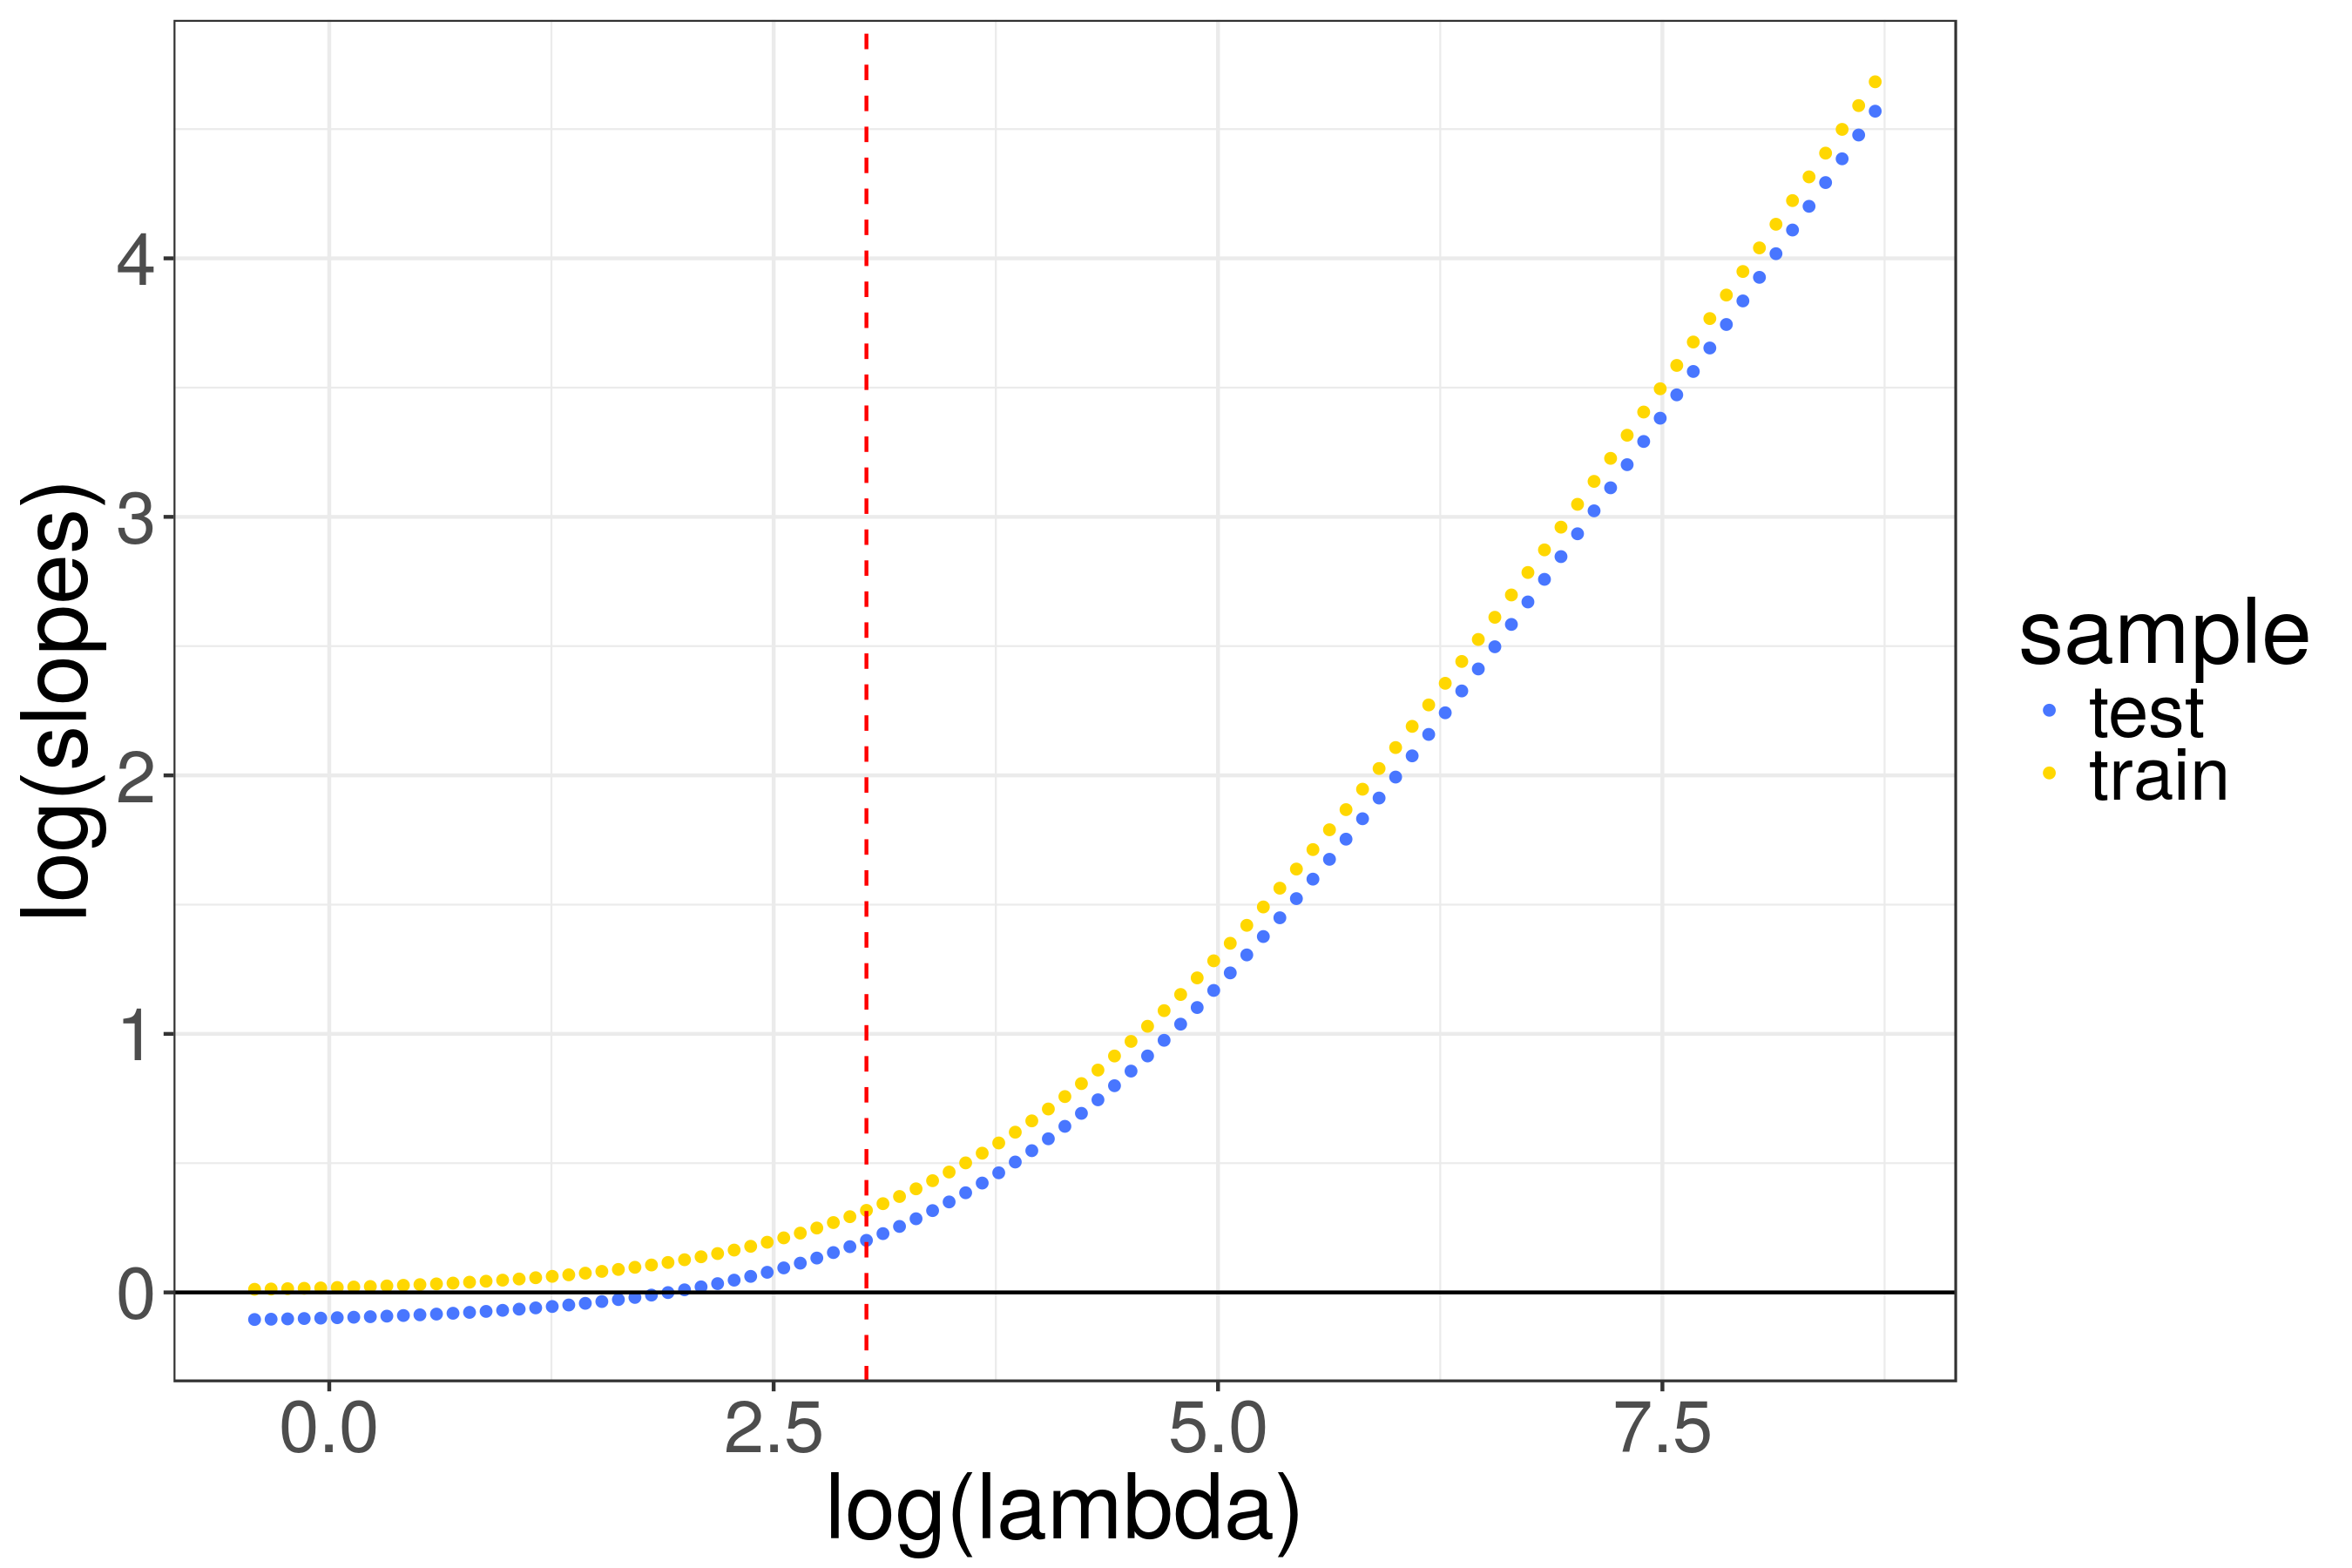
\includegraphics[width = \textwidth]{./ridge_figures/slope_vs_lambda.png}
    \subcaption{}
	\end{subfigure}
	\quad
	\begin{subfigure}[t]{0.45\textwidth}
		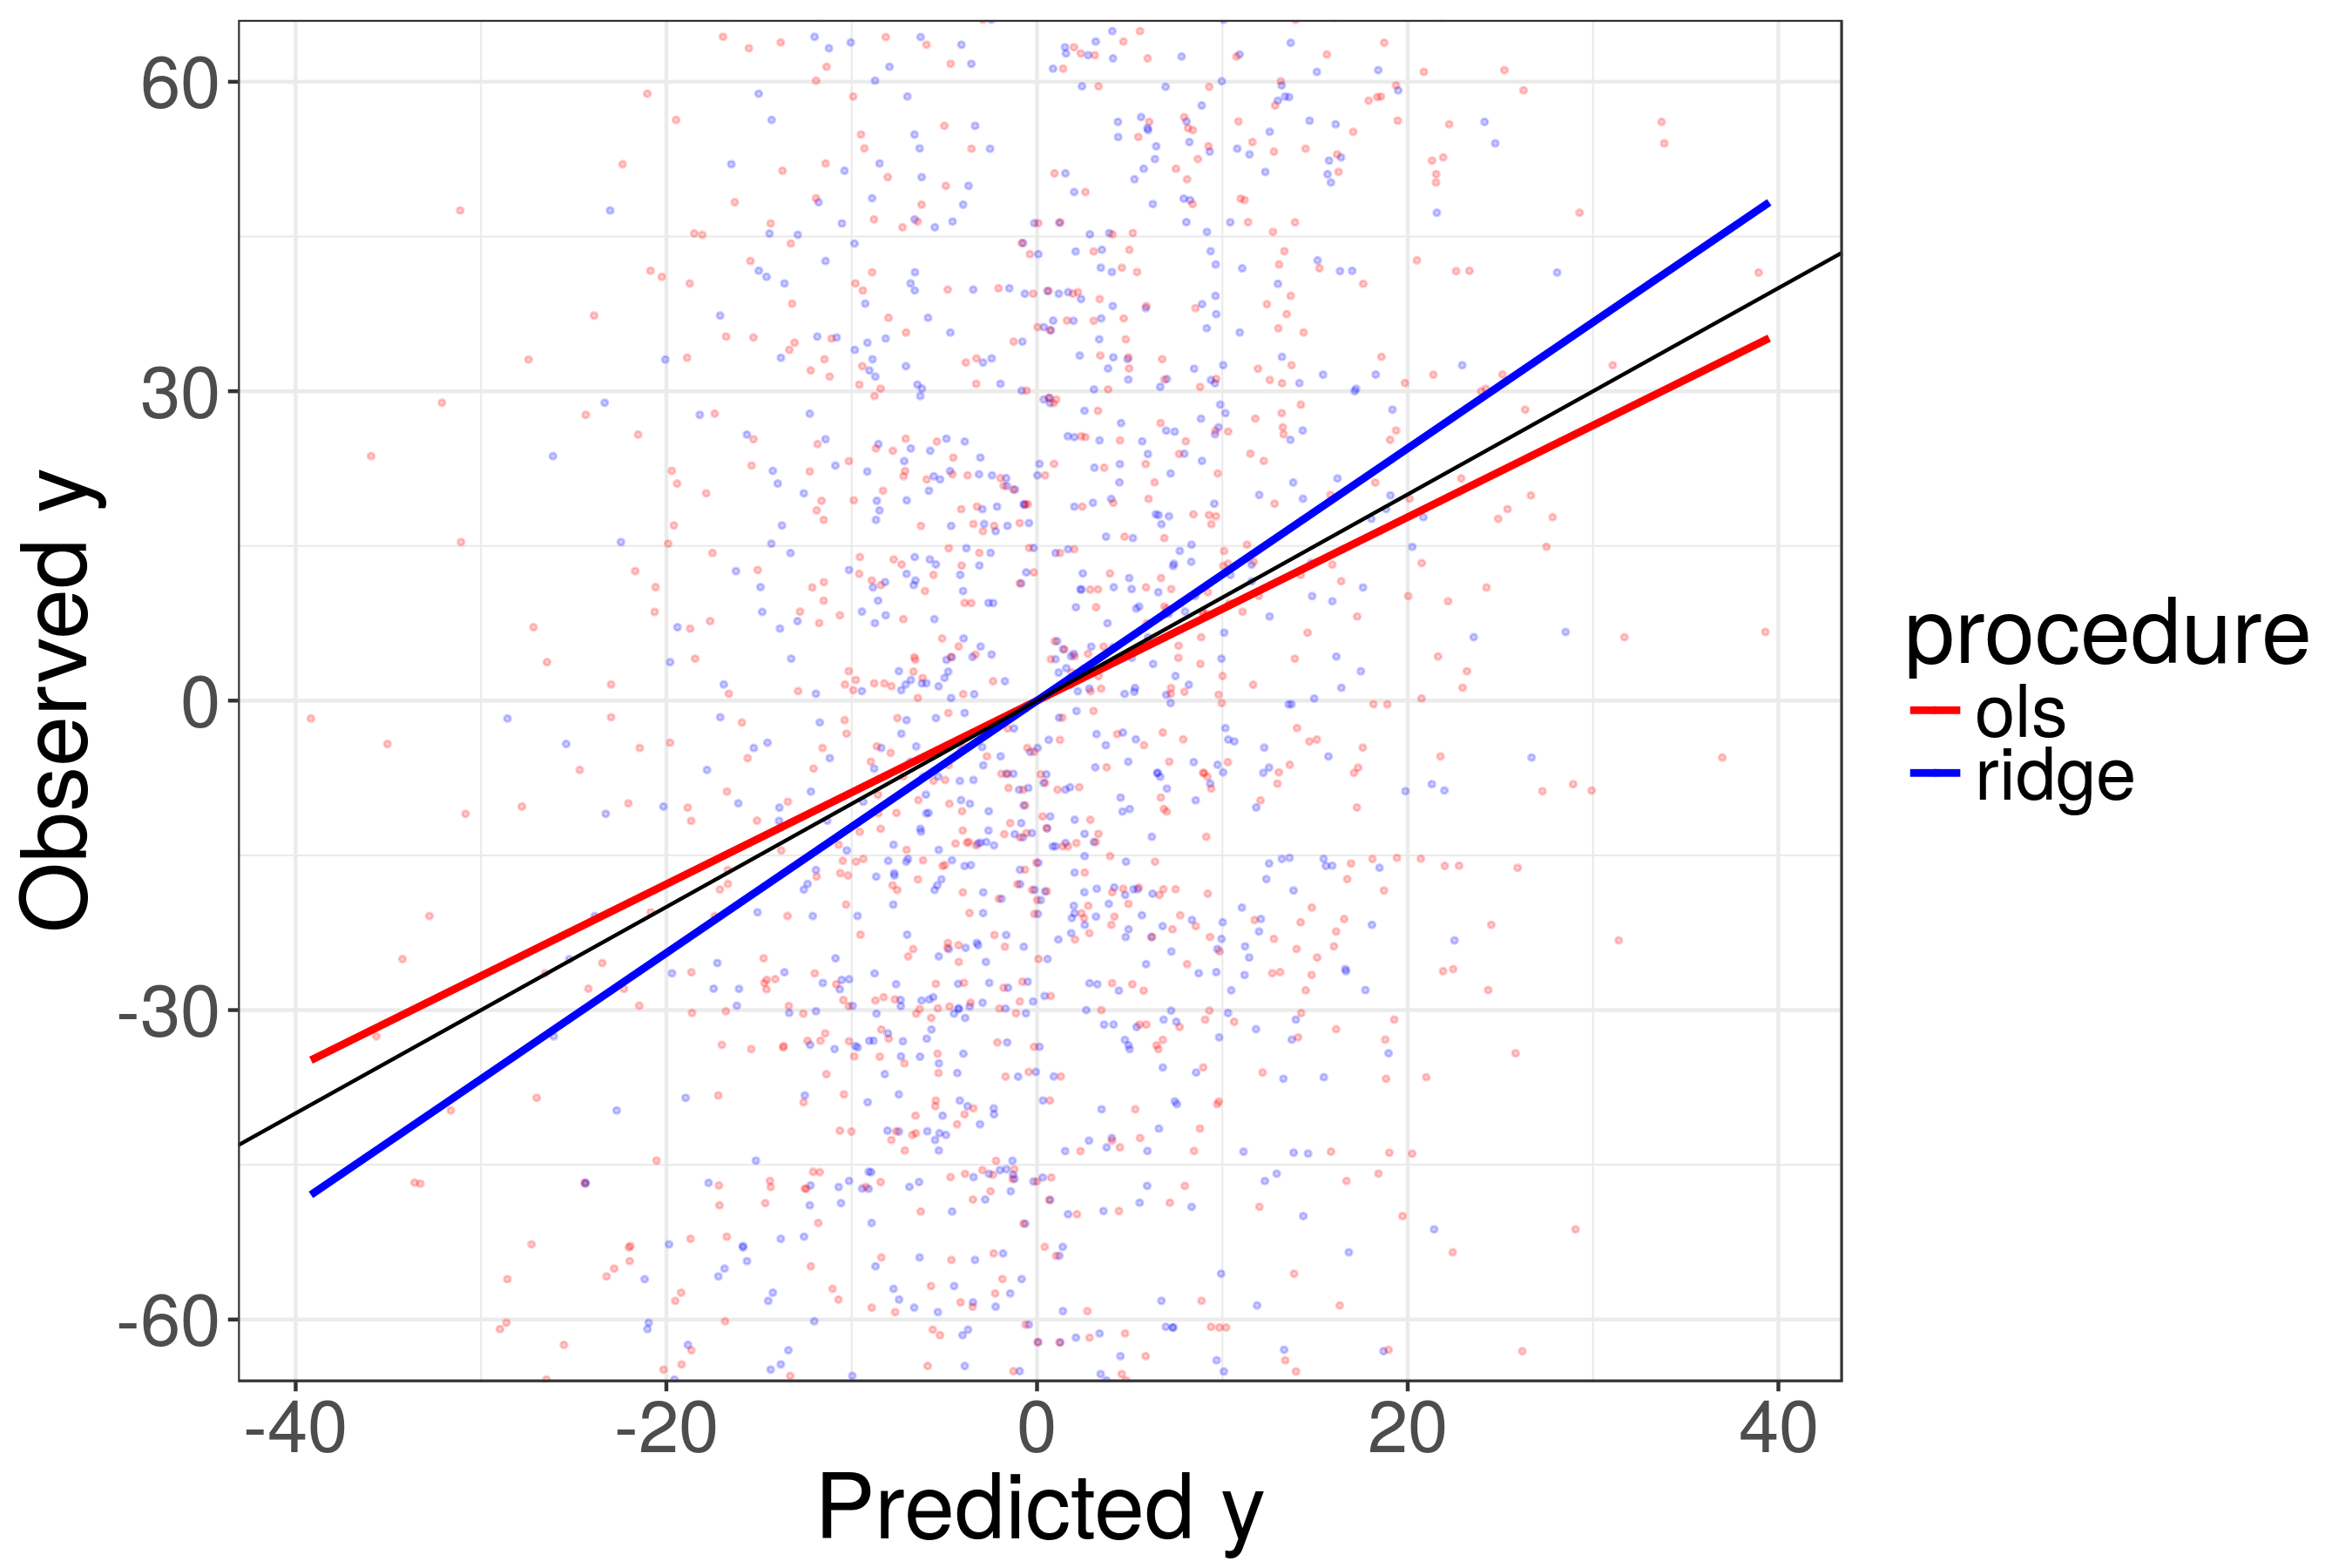
\includegraphics[width = \textwidth]{./ridge_figures/y_obs_vs_pred.png}
    \subcaption{}
	\end{subfigure}
	\caption{(a) Log(slope) of $y$ on $\hat y = x^T\hat\beta^{ridge}_\lambda$ as a function of $\log(\lambda)$.
	Vertical red line is the $\lambda$
  chosen by cross-validation. Yellow are slopes in the training sample, blue are slopes in the test sample.
  (b) Scatterplot of $(y_{new}, \hat y)$ in the test sample. Black line is the identity $y = x$ line.
	Red and blue lines are the regression
  lines of $y_{new}$ on $\hat y_{OLS}$ and $y_{new}$ on $\hat y_{ridge}$, respectively. The particular $\lambda$
	used to compute $\hat y_{ridge}$ is the same as the $\lambda$ displayed in (a). }
	\label{fig:ridge_slope_vs_lambda}
\end{figure}

We now repeat this experiment many times, each time drawing a set of 1000 training observations
$(x_{train}, y_{train})$, 10000 subsequent draws of $(x_{new}, y_{new})$, and examine $\text{slope}(y_{new}, \hat y)$, as we did above.
We wonder if this over-shrinkage by running ridge regression is a common occurrence, and if so,
whether or not choosing a pre-factor $K$ with choosing $\lambda$ can fix this problem.

In figure~\ref{fig:ridge_slope_histogram}, we display the histogram of the slopes over 500 trials. We see that for most trials, when
$\hat y$ is computed with OLS,
$\text{slope}(y_{new}, \hat y)$ is less than 1, as predicted by Copas (1983), and shrinkage is clearly needed. The distribution
of $\text{slope}(y_{new}, \hat y)$ when $\hat y$ is the ridge regression predictor seem reasonably centered at 1,
though there is a noticeable right tail of large slopes.

\begin{figure}[!h]
	\centering
	\begin{subfigure}[t]{0.45\textwidth}
		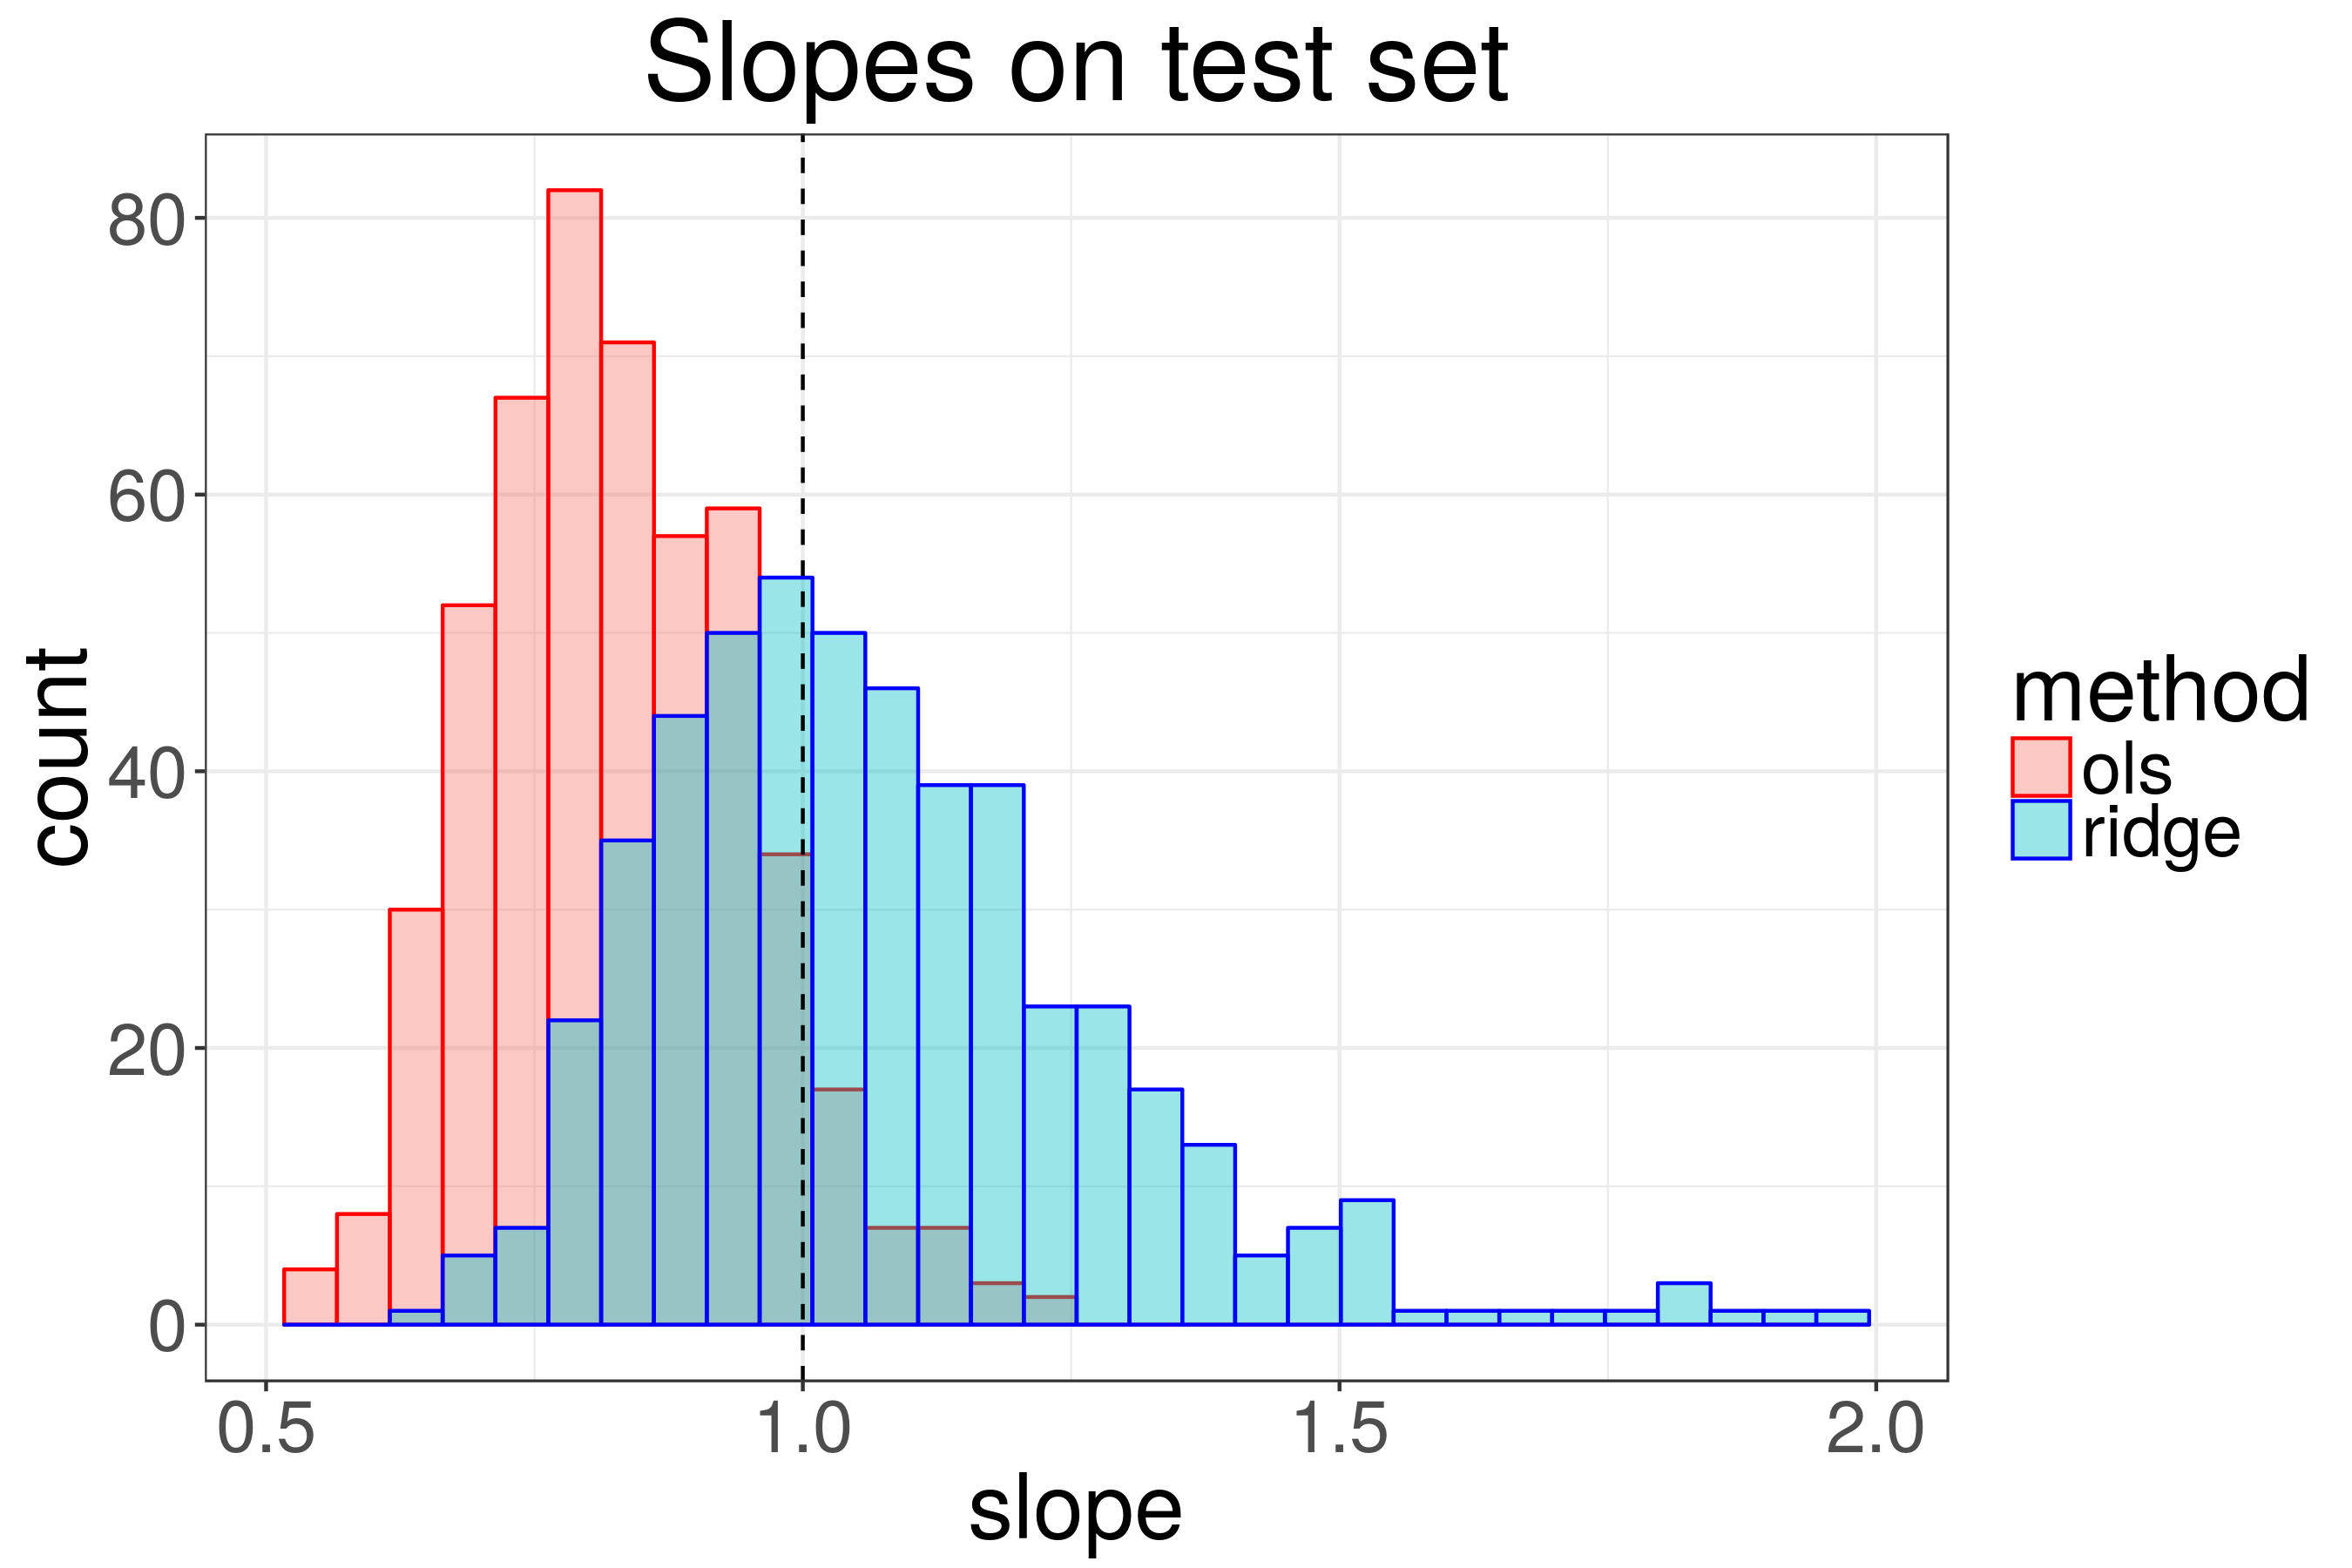
\includegraphics[width = \textwidth]{./ridge_figures/slope_distr_hist_sigma50.png}
	\end{subfigure}
  \caption{Histogram of $\text{slope}(y_{new}, \hat y)$ over 500 trials. Red are slopes when $\hat y$ is obtained by OLS. Blue
  are slopes when $\hat y$ are obtained by ridge regression and cross-validation selected $\lambda$. }
  \label{fig:ridge_slope_histogram}
\end{figure}

We then examine the performance of choosing a pre-factor $K$.
In figure~\ref{fig:ridge_results_fixed_sigma}a, we compare the distribution of slopes when choosing $K$
to the slope distribution
of OLS and ridge regression. We see that choosing this factor $K$ in addition to choosing $\lambda$ indeed lowers
the slope, but by a bit too much. For all the methods of choosing $K$, the median slopes are again below 1,
though they are closer to 1 than the OLS slopes. The median slope of the Copas procedure is very close to 1,
which is unsurprising given that the simulation setup is the same as in Copas (1983); however, the median slope of our
two-step procedure is also not far from one.

We then compare the distribution of test set MSPEs in figure~\ref{fig:ridge_results_fixed_sigma}b, and we find that
$K$ selection does not seem to yield significant improvements. The median MSPE for selecting $K$ jointly
was slightly larger than the median MSPE for ridge regression, while the median MSPE was slightly smaller for
the Copas and the two-step procedure. The median MSPEs for all the types of shrinkage considered here,
ridge, Copas, joint or two-step $K$ selection, was smaller than simple OLS, however.
In sum, both ridge
regression and our addition of $K$ improved upon OLS, but the selection of $K$ in the two-step procedure
gave only slight improvements over ridge regression.

\begin{figure}[!h]
	\centering
	\begin{subfigure}[t]{0.45\textwidth}
		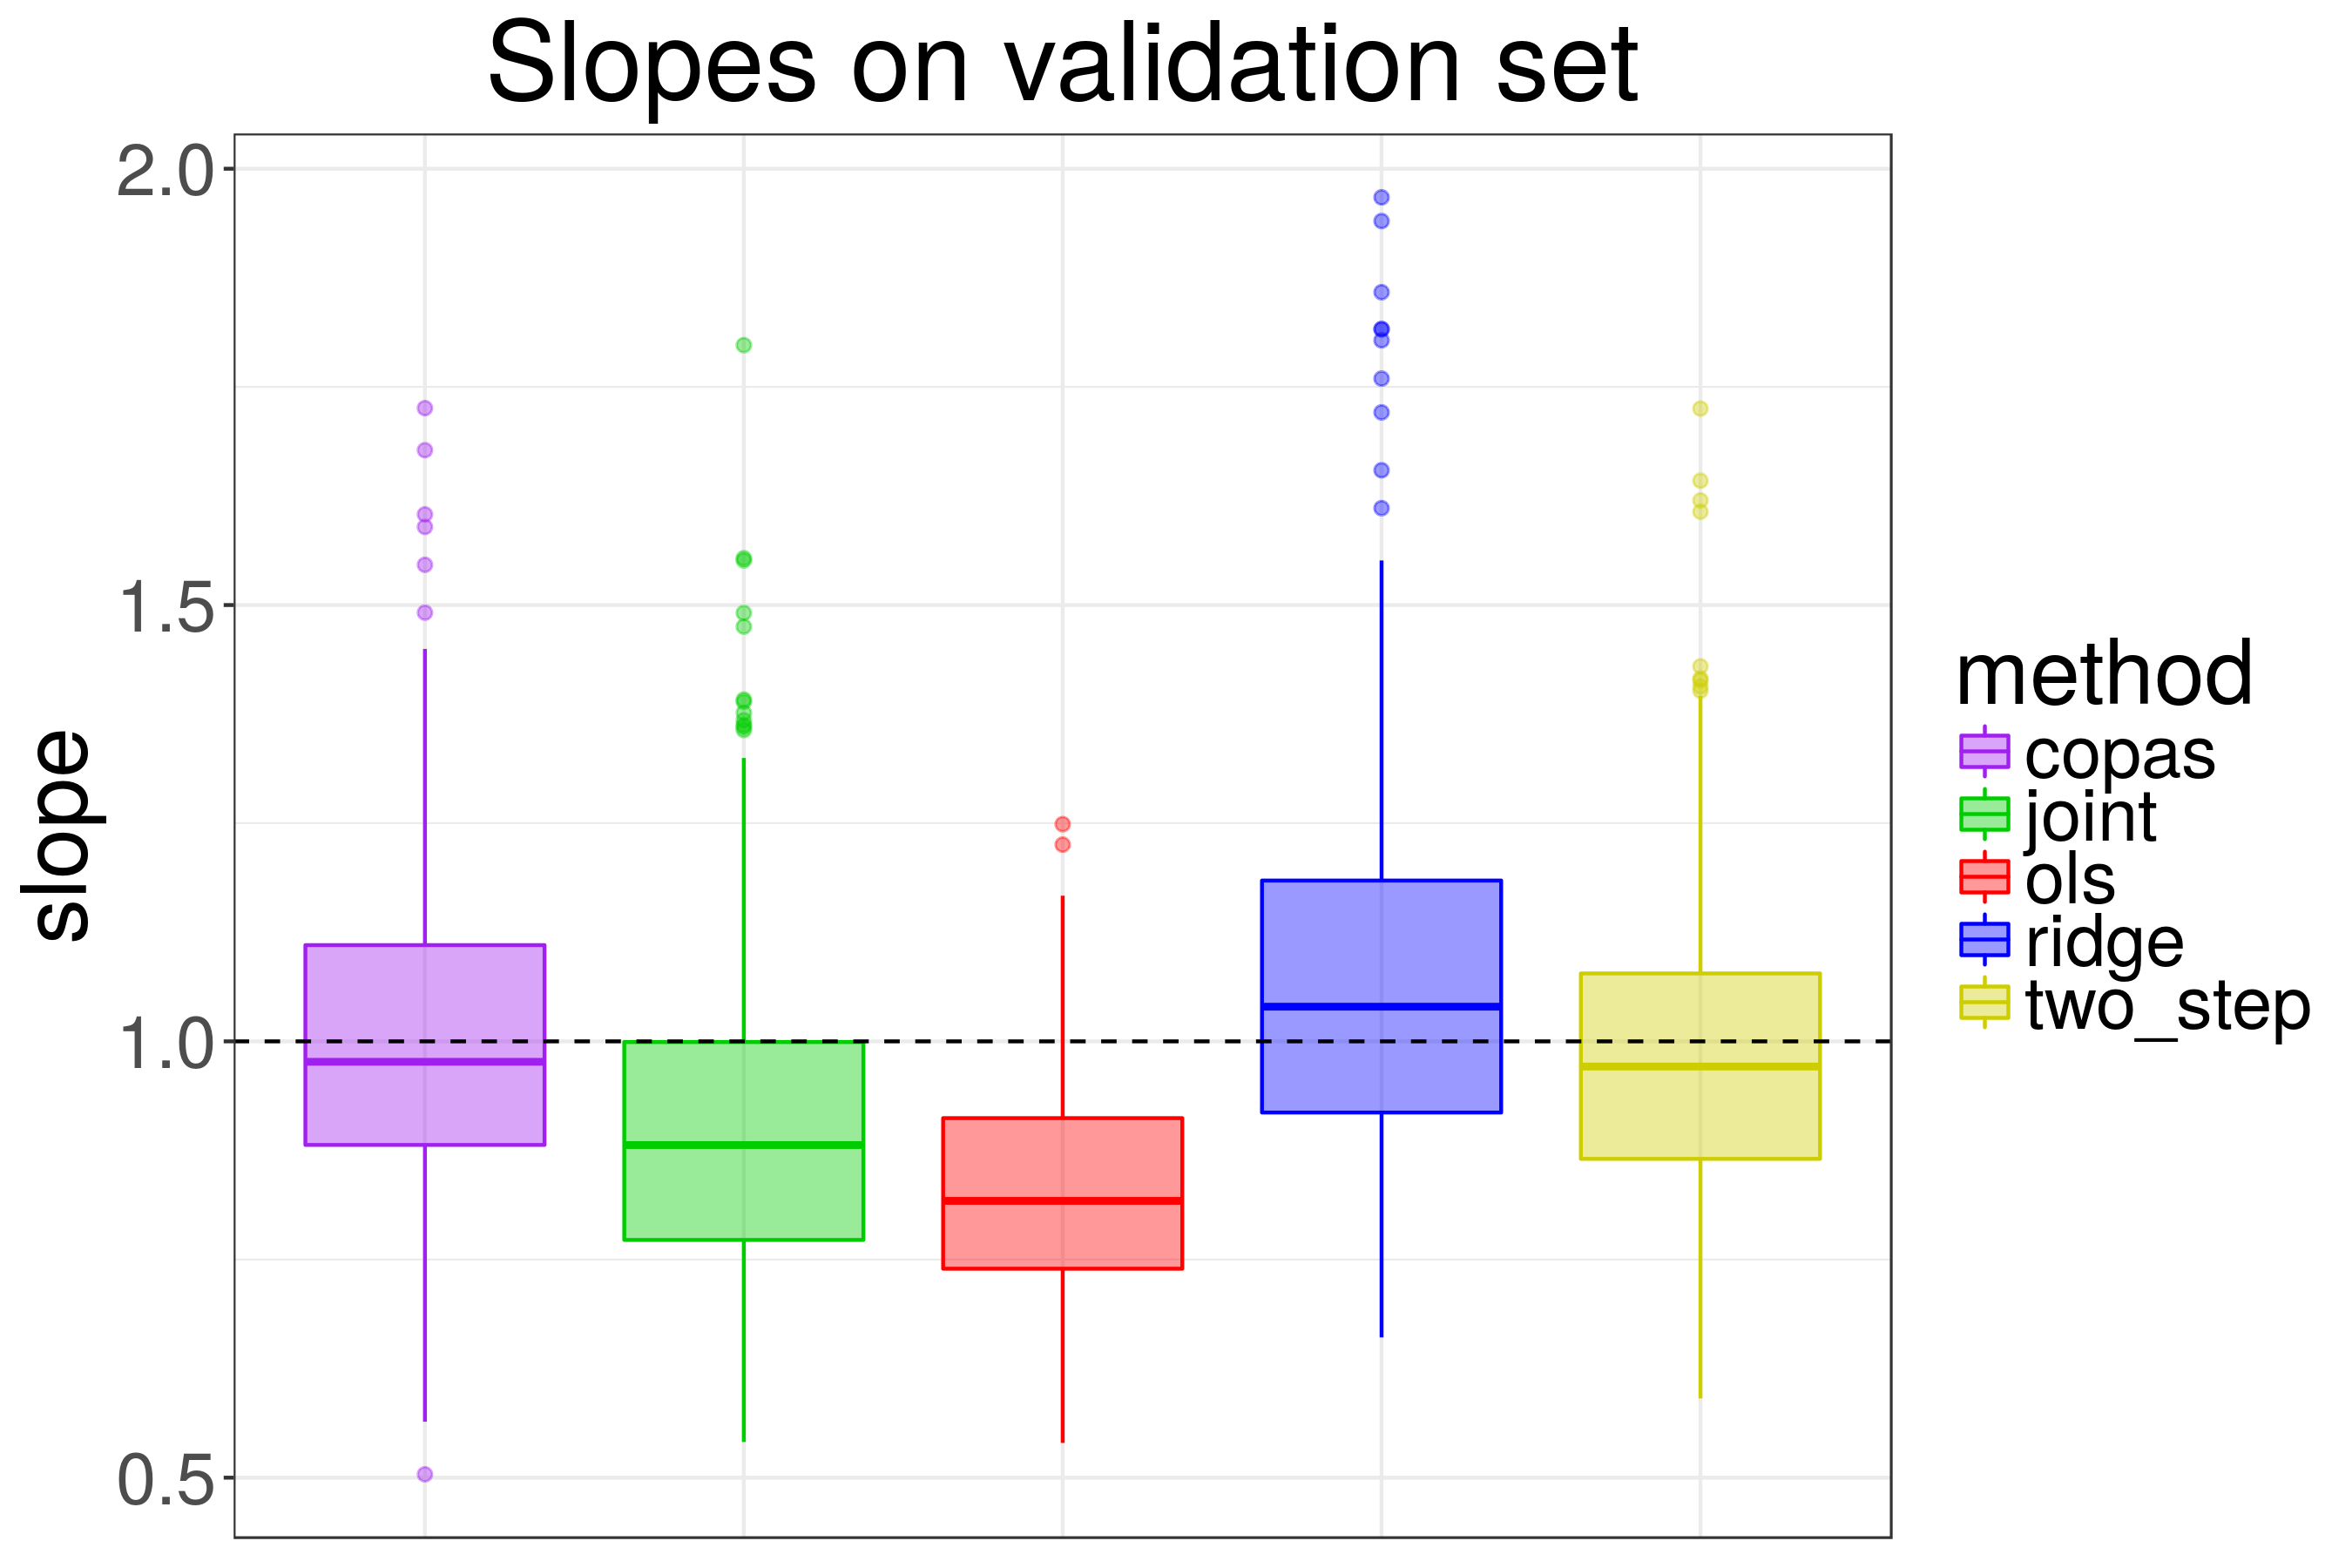
\includegraphics[width = \textwidth]{./ridge_figures/slope_distr_sigma50.png}
	\end{subfigure}
  \begin{subfigure}[t]{0.45\textwidth}
    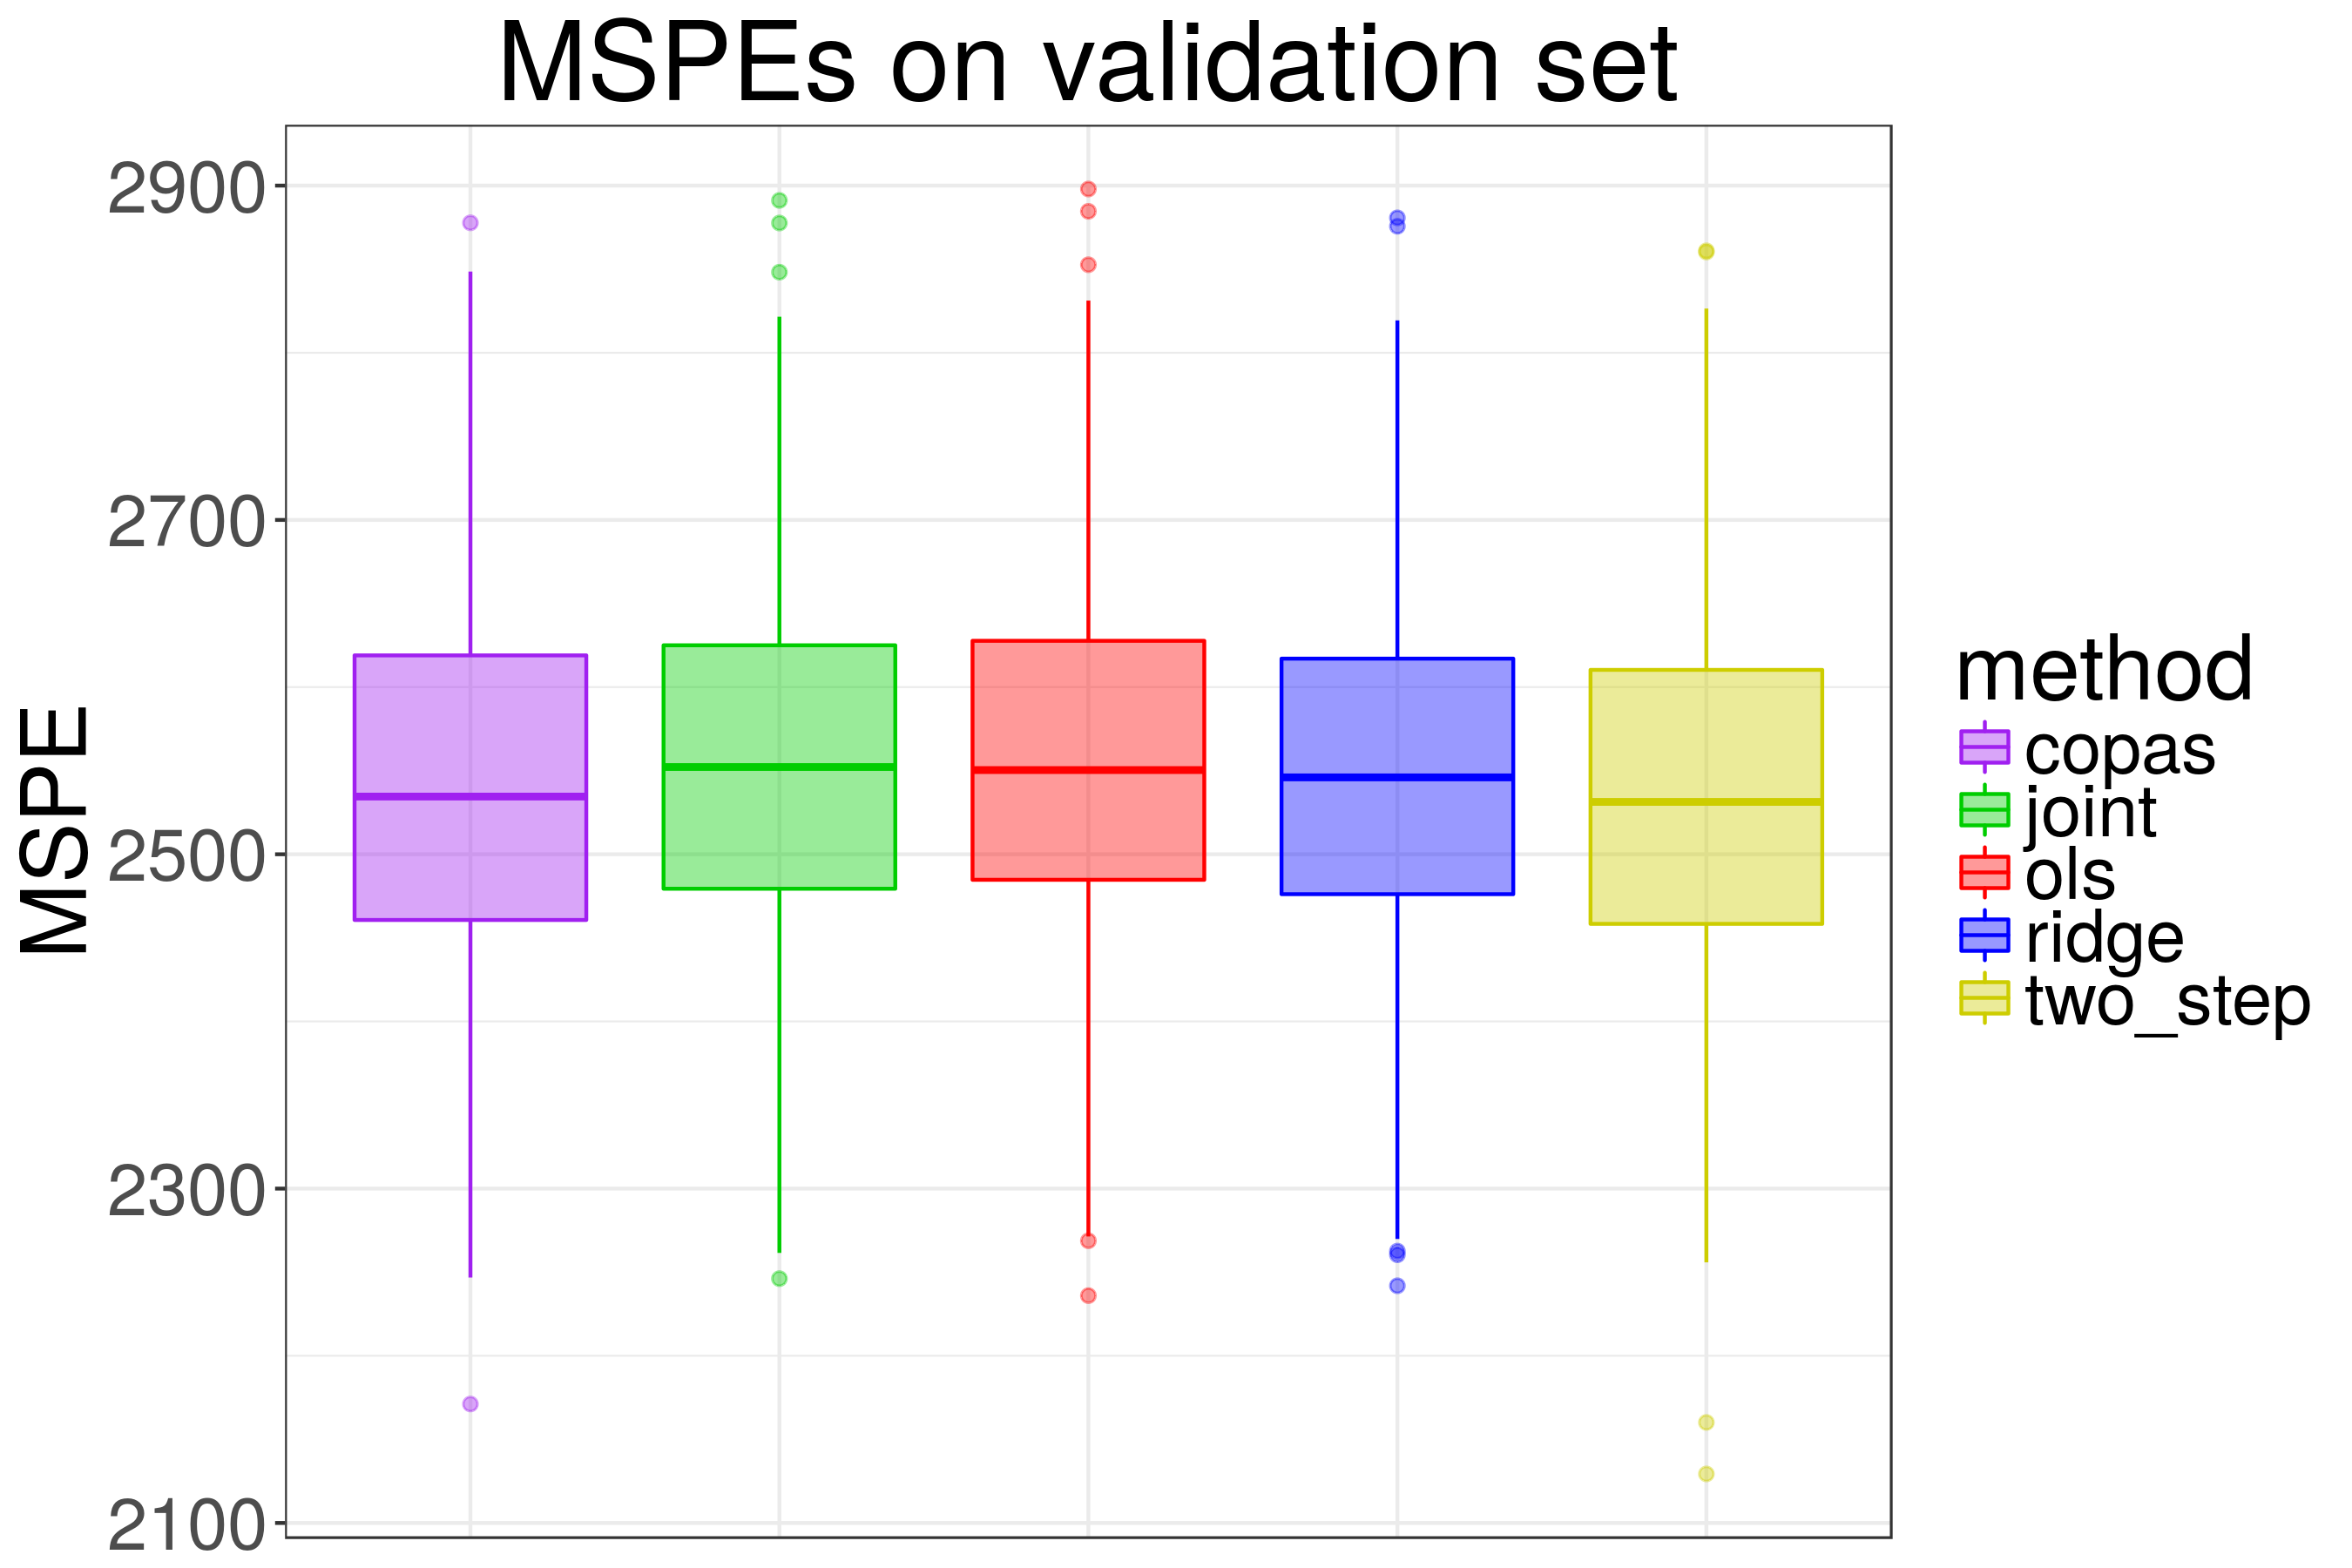
\includegraphics[width = \textwidth]{./ridge_figures/mspe_distr_sigma50.png}
  \end{subfigure}
  \caption{(a) Distribution of $\text{slope}(y_{new}, \hat y)$ for $\hat y$ computed with OLS, OLS with Copas $K$,
	ridge regression, joint $(\lambda, K)$ selection, and two-step $(\lambda, K)$ selection;
	(b) Distribution of MSPEs in the test set, relative to OLS.
	In this plot we set $\sigma = 50$}
	\label{fig:ridge_results_fixed_sigma}
\end{figure}

\noindent{\bf Varying the noise: }\par
Next, we consider what happens as we vary the noise in our simulations. The experiments above had $\sigma$ set at 50; below,
we rerun the experiment above (each experiment again with 500 trials) for several different $\sigma$s.
In figure \ref{fig:ridge_results_varying_sigma}a, we plot the median $\text{slope}(y_{new}, \hat y)$ for the 500 trials against $\sigma$.
We see that the slope for OLS starts near 1 when $\sigma$ is small, and decays rapidly. This makes sense: as our data
become more noisy, OLS overfits to the noise in the training set, and hence its performance on the test set suffers.
Ridge regression, with its regularization term, avoids this overfitting problem, as its median slopes are consistently above 1 for
all $\sigma$ -- while it does consistently {\itshape over-shrink}, the performance does not seem to become worse
with $\sigma$, like for OLS. We hoped that choosing $K$ would fix the over-shrinking problem, but choosing
$K$ seemed to overcompensate; the slopes become consistently less than 1. However, it is encouraging that again, the slopes
do not seem to become as bad as OLS with larger $\sigma$.

Finally, figure \ref{fig:ridge_results_varying_sigma}b plots the MSPE relative to OLS.
While OLS does better for smaller $\sigma$, regularization is needed for noisy problems, and doing ridge regression and/or
choosing $K$ improved on MSPE. The two-step procedure had the smallest median MSPE among all the methods,
for all but the noisiest case.

\begin{figure}[!h]
	\centering
	\begin{subfigure}[t]{0.45\textwidth}
		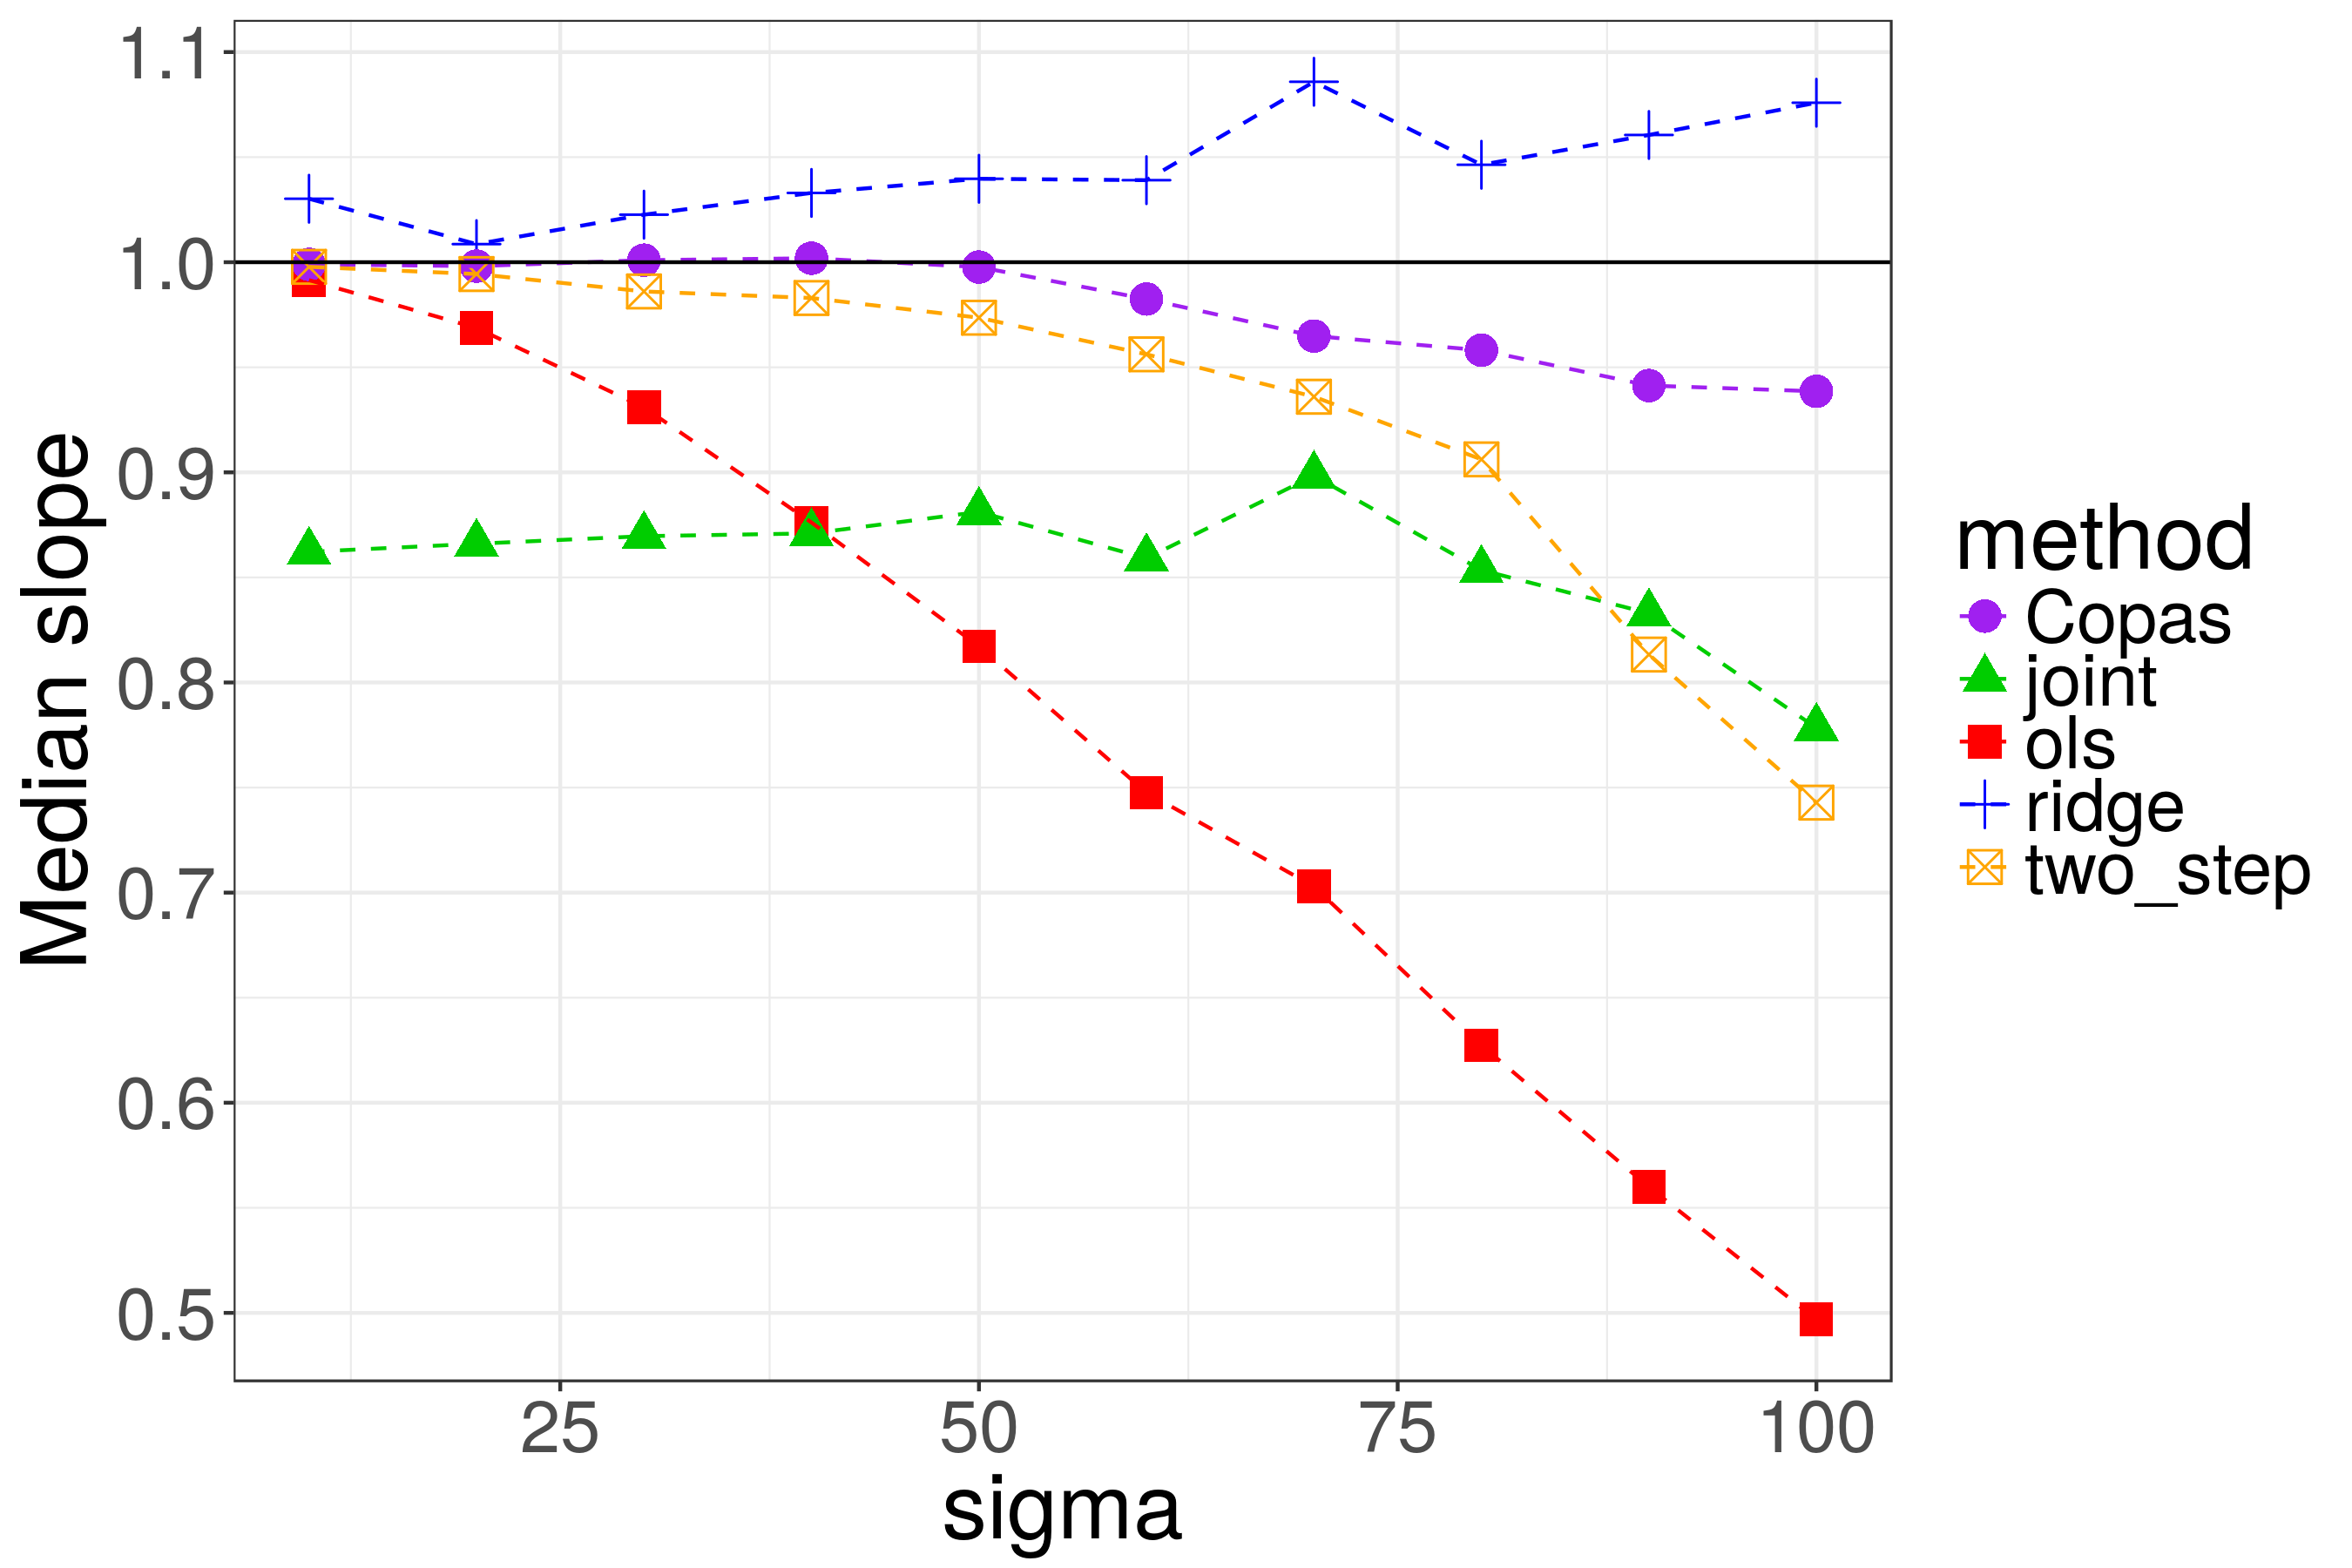
\includegraphics[width = \textwidth]{./ridge_figures/slopes_over_sigmas.png}
	\end{subfigure}
  \begin{subfigure}[t]{0.45\textwidth}
    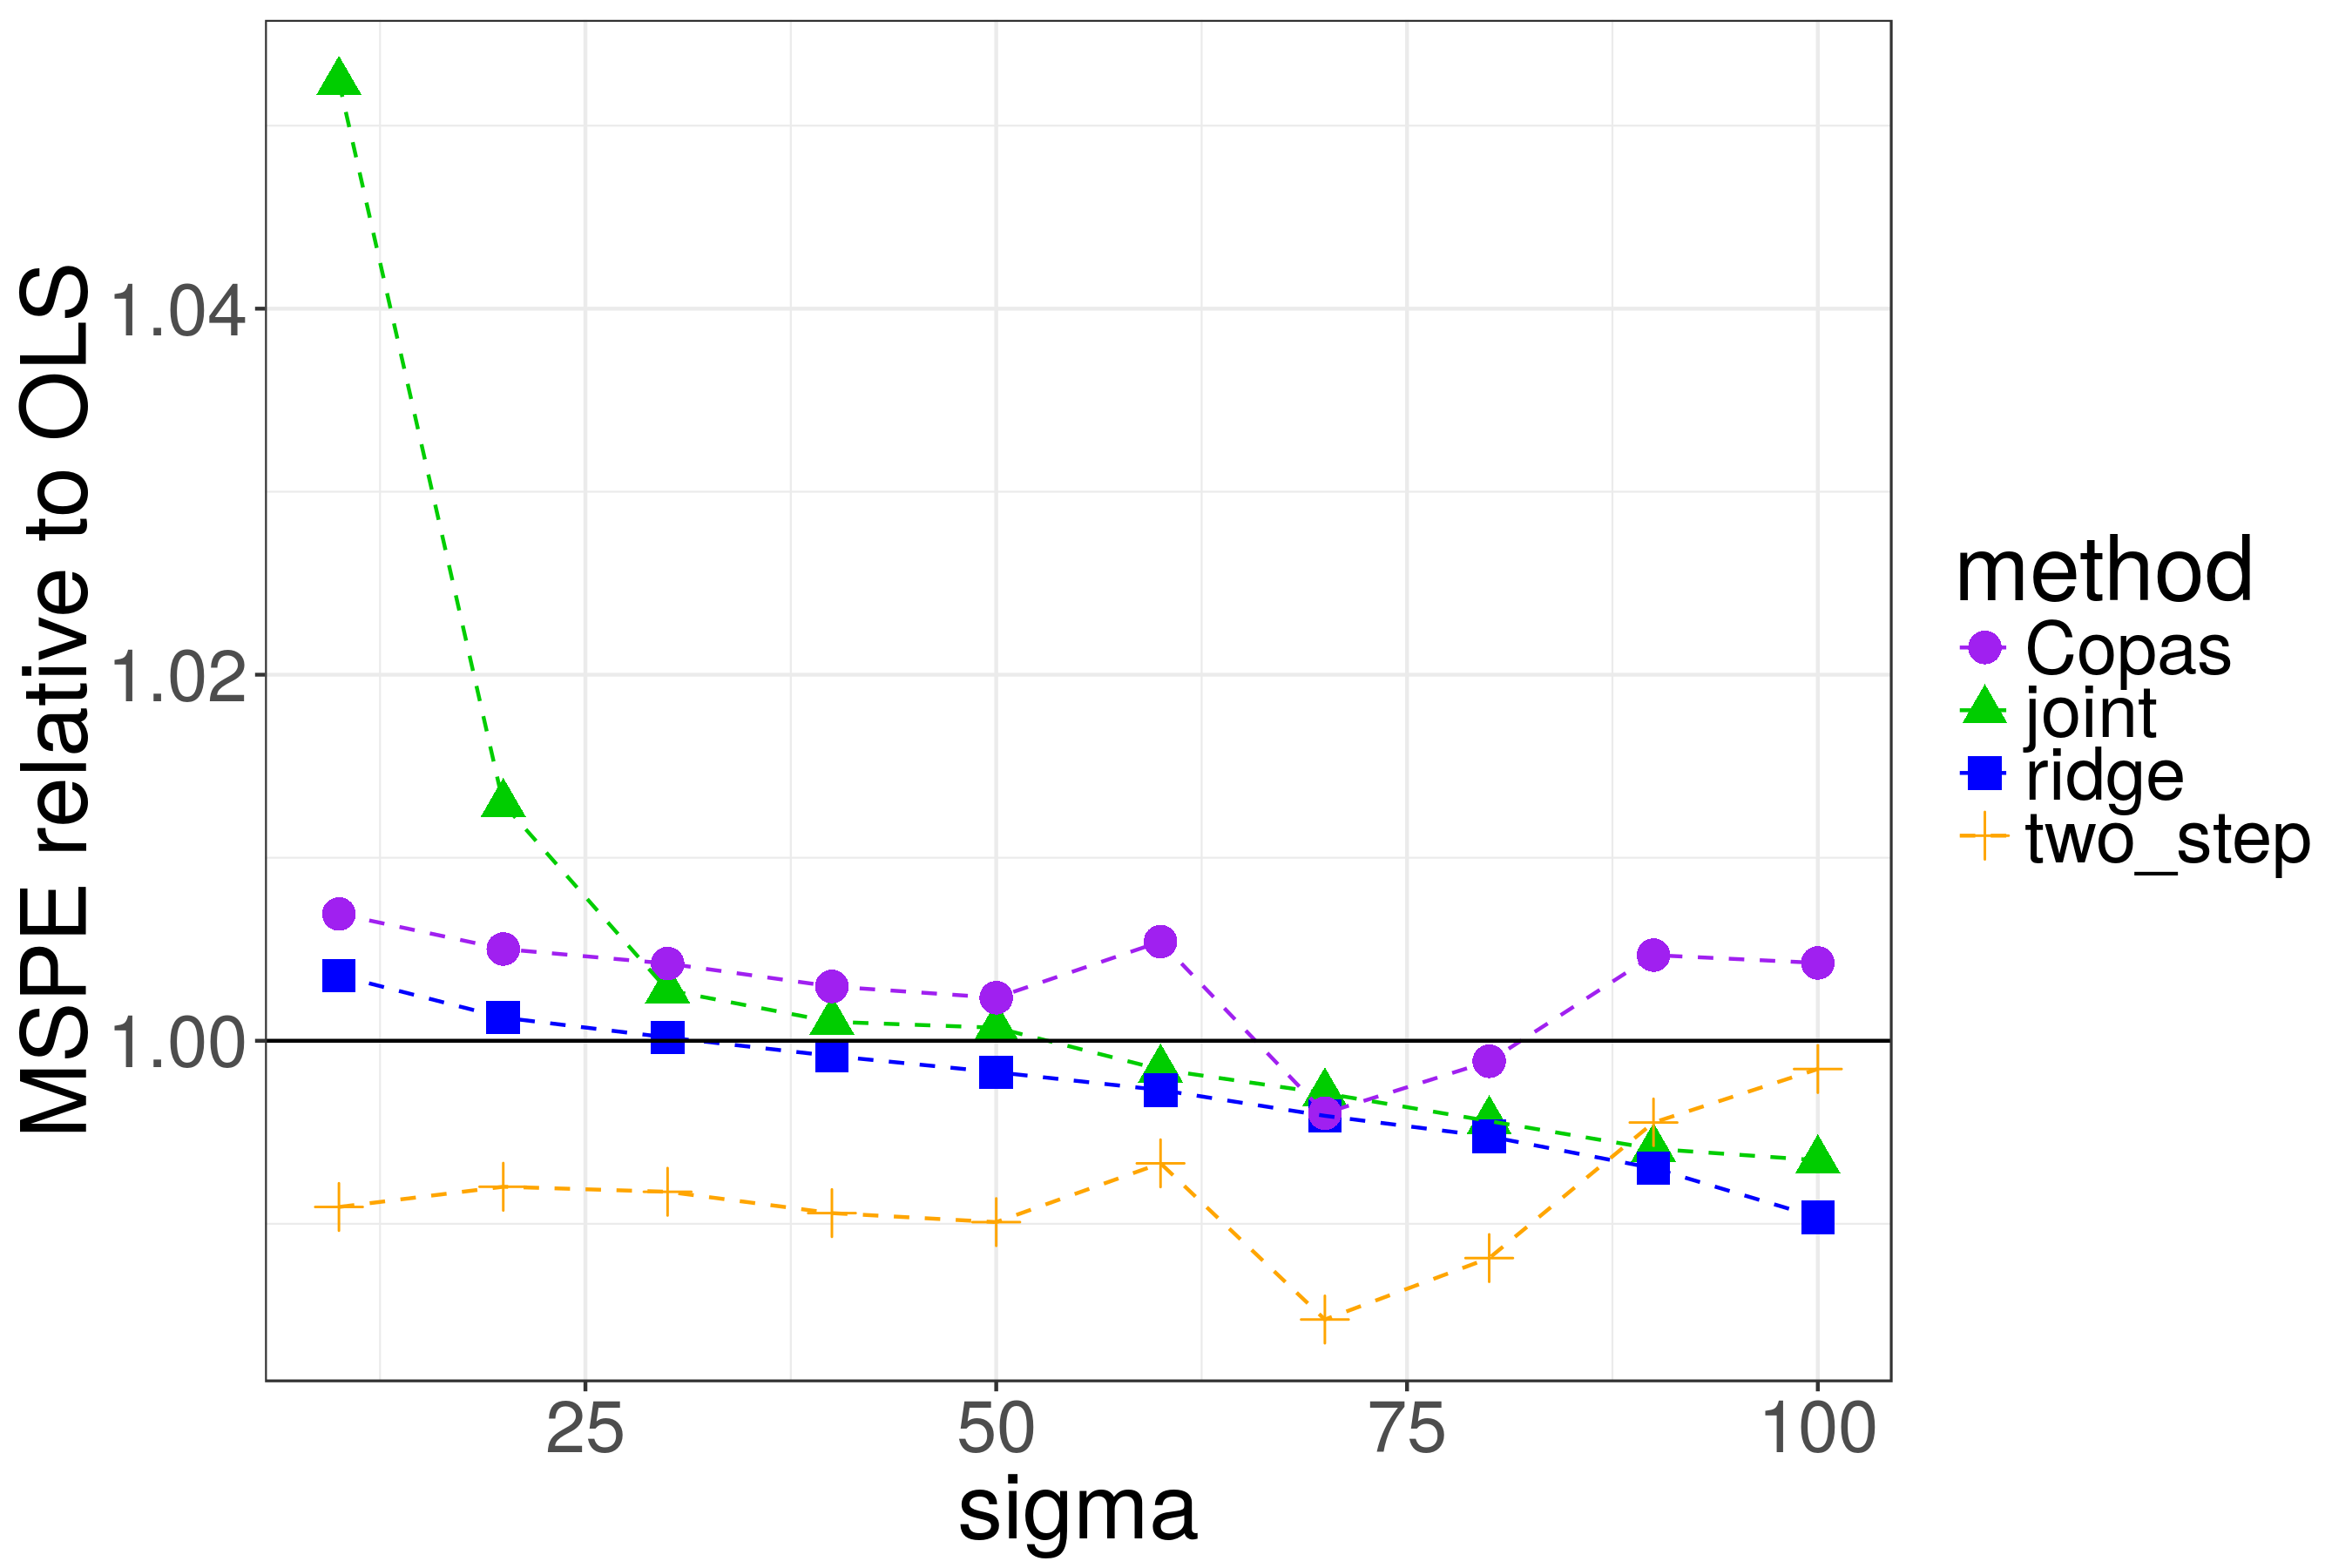
\includegraphics[width = \textwidth]{./ridge_figures/mspe_over_sigmas.png}
  \end{subfigure}
  \caption{(a) Median $\text{slope}(y_{new}, \hat y)$ over 500 trials, as a function of the noise $\sigma$, (b)
	median MSPEs on the test set, relative to OLS, as a function of the noise $\sigma$.  }
	\label{fig:ridge_results_varying_sigma}
\end{figure}


\subsection{LASSO Simulation Study}
Like in the ridge regression analysis,
we use a simulation study to examine the predictive performance of choosing $K$ in addition to $\lambda$ when running
LASSO.

% The lasso problem solves
% \begin{align}
% 	\hat\beta^{lasso}_\lambda = \arg\min_{\beta} \|y - X\beta\|^2 + \lambda \|\beta\|_1
% \end{align}
% for $X$ and $y$ in a training set. Given a new draw $x_{new}$, we can predict $y_{new}$ with $\hat y = x_{new}^T\hat\beta^{lasso}_\lambda$. Traditionally,
% $\lambda$ is chosen by cross-validation. Like in our ridge regression case, we can ask whether our lasso predictions
% $\hat y = x_{new}\beta^{lasso}_{\lambda}$ are too large or too small. If further shrinkage (or inflation) is needed, we can choose
% $K$ and predict with $\hat y = K x_{new}\beta_{\lambda}$. We again propose to jointly choose $\lambda$ and $k$
% by cross-validation,
% and compare the performance of this method against the traditional LASSO procedure where only $\lambda$ is chosen.

\subsubsection{Simulation Setup}
The set-up is similar to Copas (1983), except the number of features $p$ is larger than the number of
observations in our training set $n$,
and we enforce the true $\beta$ to be sparse. We pick a matrix $X_{train} \in \mathbb{R}^{n \times p}$, and
$\beta_{full} \in \mathbb{R}^p$, to be fixed for the remainder of this analysis. Let $s$ be the sparsity parameter, and let
$\beta_s$ be $\beta_{full}$ but with its first $p - s$ entries set to 0.
We then generate $y_{train} \sim \mathcal{N}(X_{train}\beta_s, \sigma^2 I_{n\times n})$.
We set the size of our training set $n$ to 200, and set $p$ to 1000.
We subsequently draw a test set, whose features $x_{new}$ are drawn from a zero mean multivariate normal distribution with
covariance given by the empirical covariance of $X_{train}$; $y_{new}$ are then drawn $\mathcal{N}(x_{new}\beta_s, \sigma^2)$.
We set the size of our test set to be 1000. We again examine $\text{slope}(y_{new}, \hat y)$ and
$\text{MSPE}(y_{new}, \hat y)$ across many trials of this data generation procedure.


\subsubsection{Simulation Results}

Using similar reasoning as in the ridge regression case, whether our LASSO regression predictor
$\hat y = x^T \hat\beta^{lasso}_\lambda$ needs to be shrunk or inflated depends
on our choice of $\lambda$. In figure
\ref{fig:lasso_results_fixed}a, where we show $\text{slope}(y_{new}, \hat y)$ as a function of $\lambda$.
When $\lambda$ is small, we are in the OLS regime, and our slope is less than 1 as expected, and shrinkage is needed;
when $\lambda$ is large, the slope is greater than 1, and inflation is needed. For this particular experiment,
cross-validation chose a $\lambda$ that returned a slope greater than 1, and inflating our
predictions may provide better estimates of $y_{new}$.

% Figure \ref{fig:lasso_results_fixed}b shows a scatter-plot of $y_{new}$ against $\hat y$, for $\hat y$ obtained with LASSO with
% CV selected $\lambda$, and for $\hat y$ with $K$ and $\lambda$ jointly CV selected. The blue line is the regression
% line of $y_{new}$ on $\hat y$ for when only $\lambda$ is selected, and we see that the slope is above 1, and the LASSO over-shrunk.

\begin{figure}[!h]
	\centering
	\begin{subfigure}[t]{0.45\textwidth}
		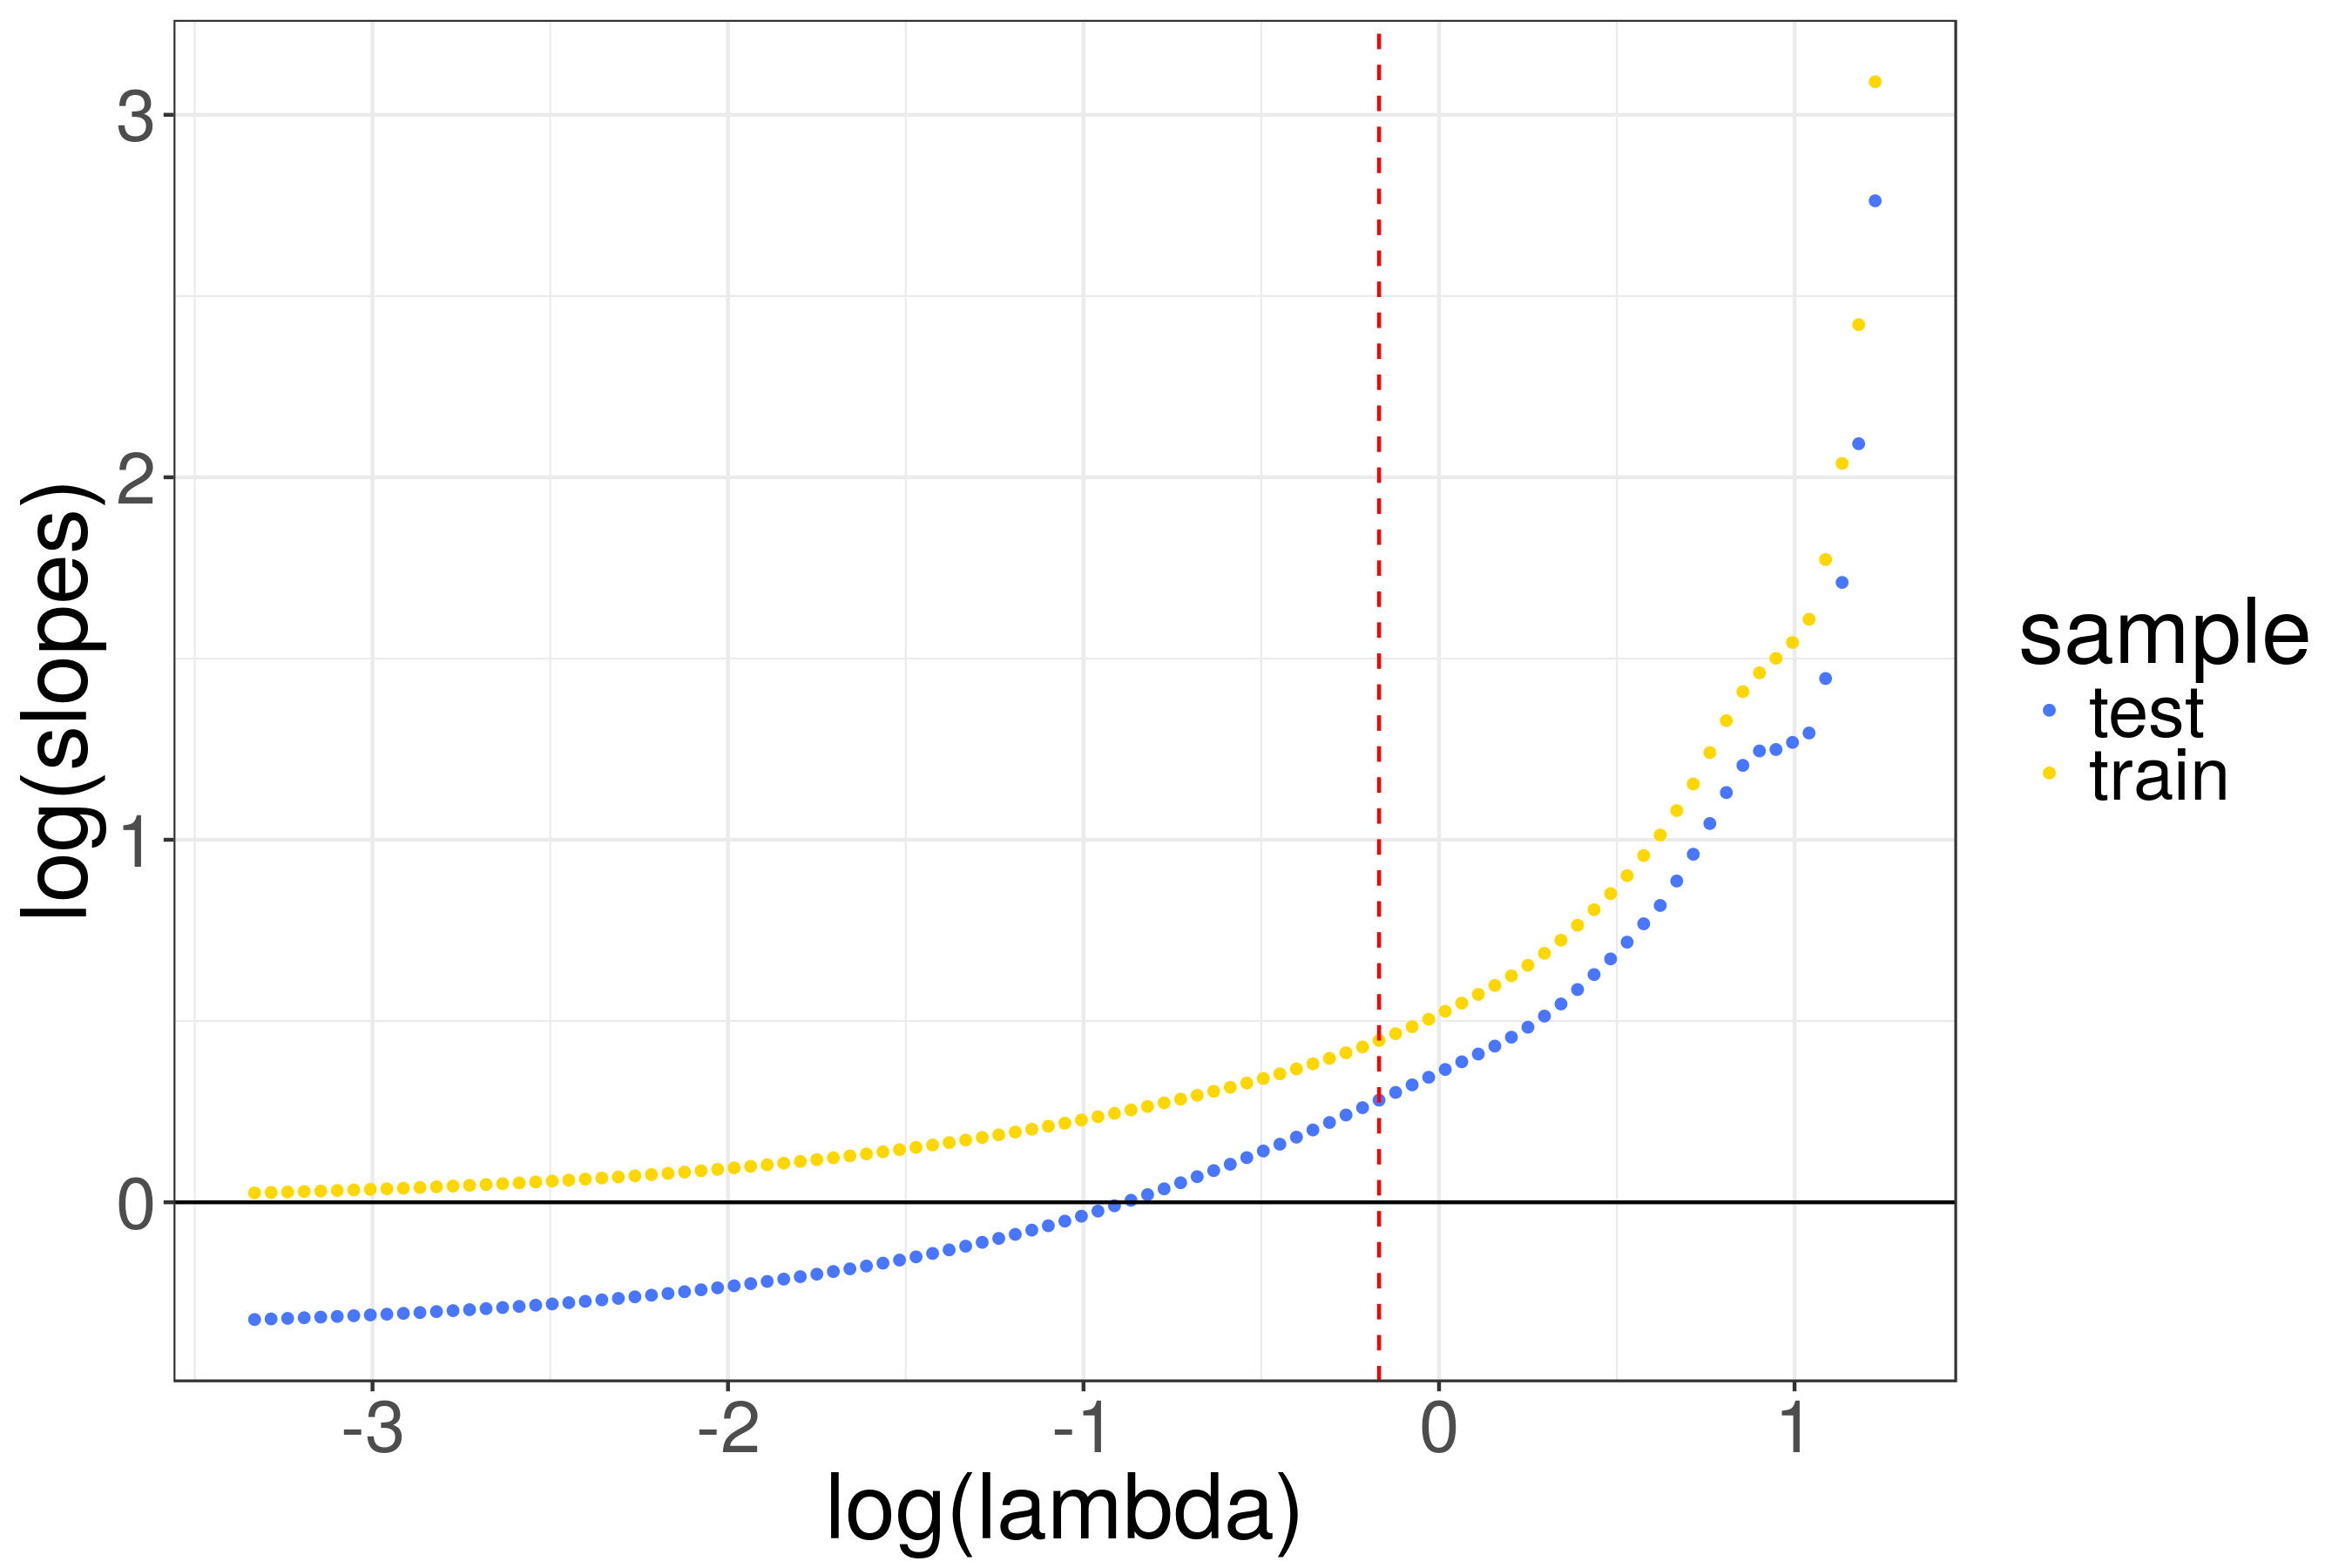
\includegraphics[width = \textwidth]{./lasso_figures/slope_vs_lambda.png}
	\end{subfigure}
  \begin{subfigure}[t]{0.45\textwidth}
    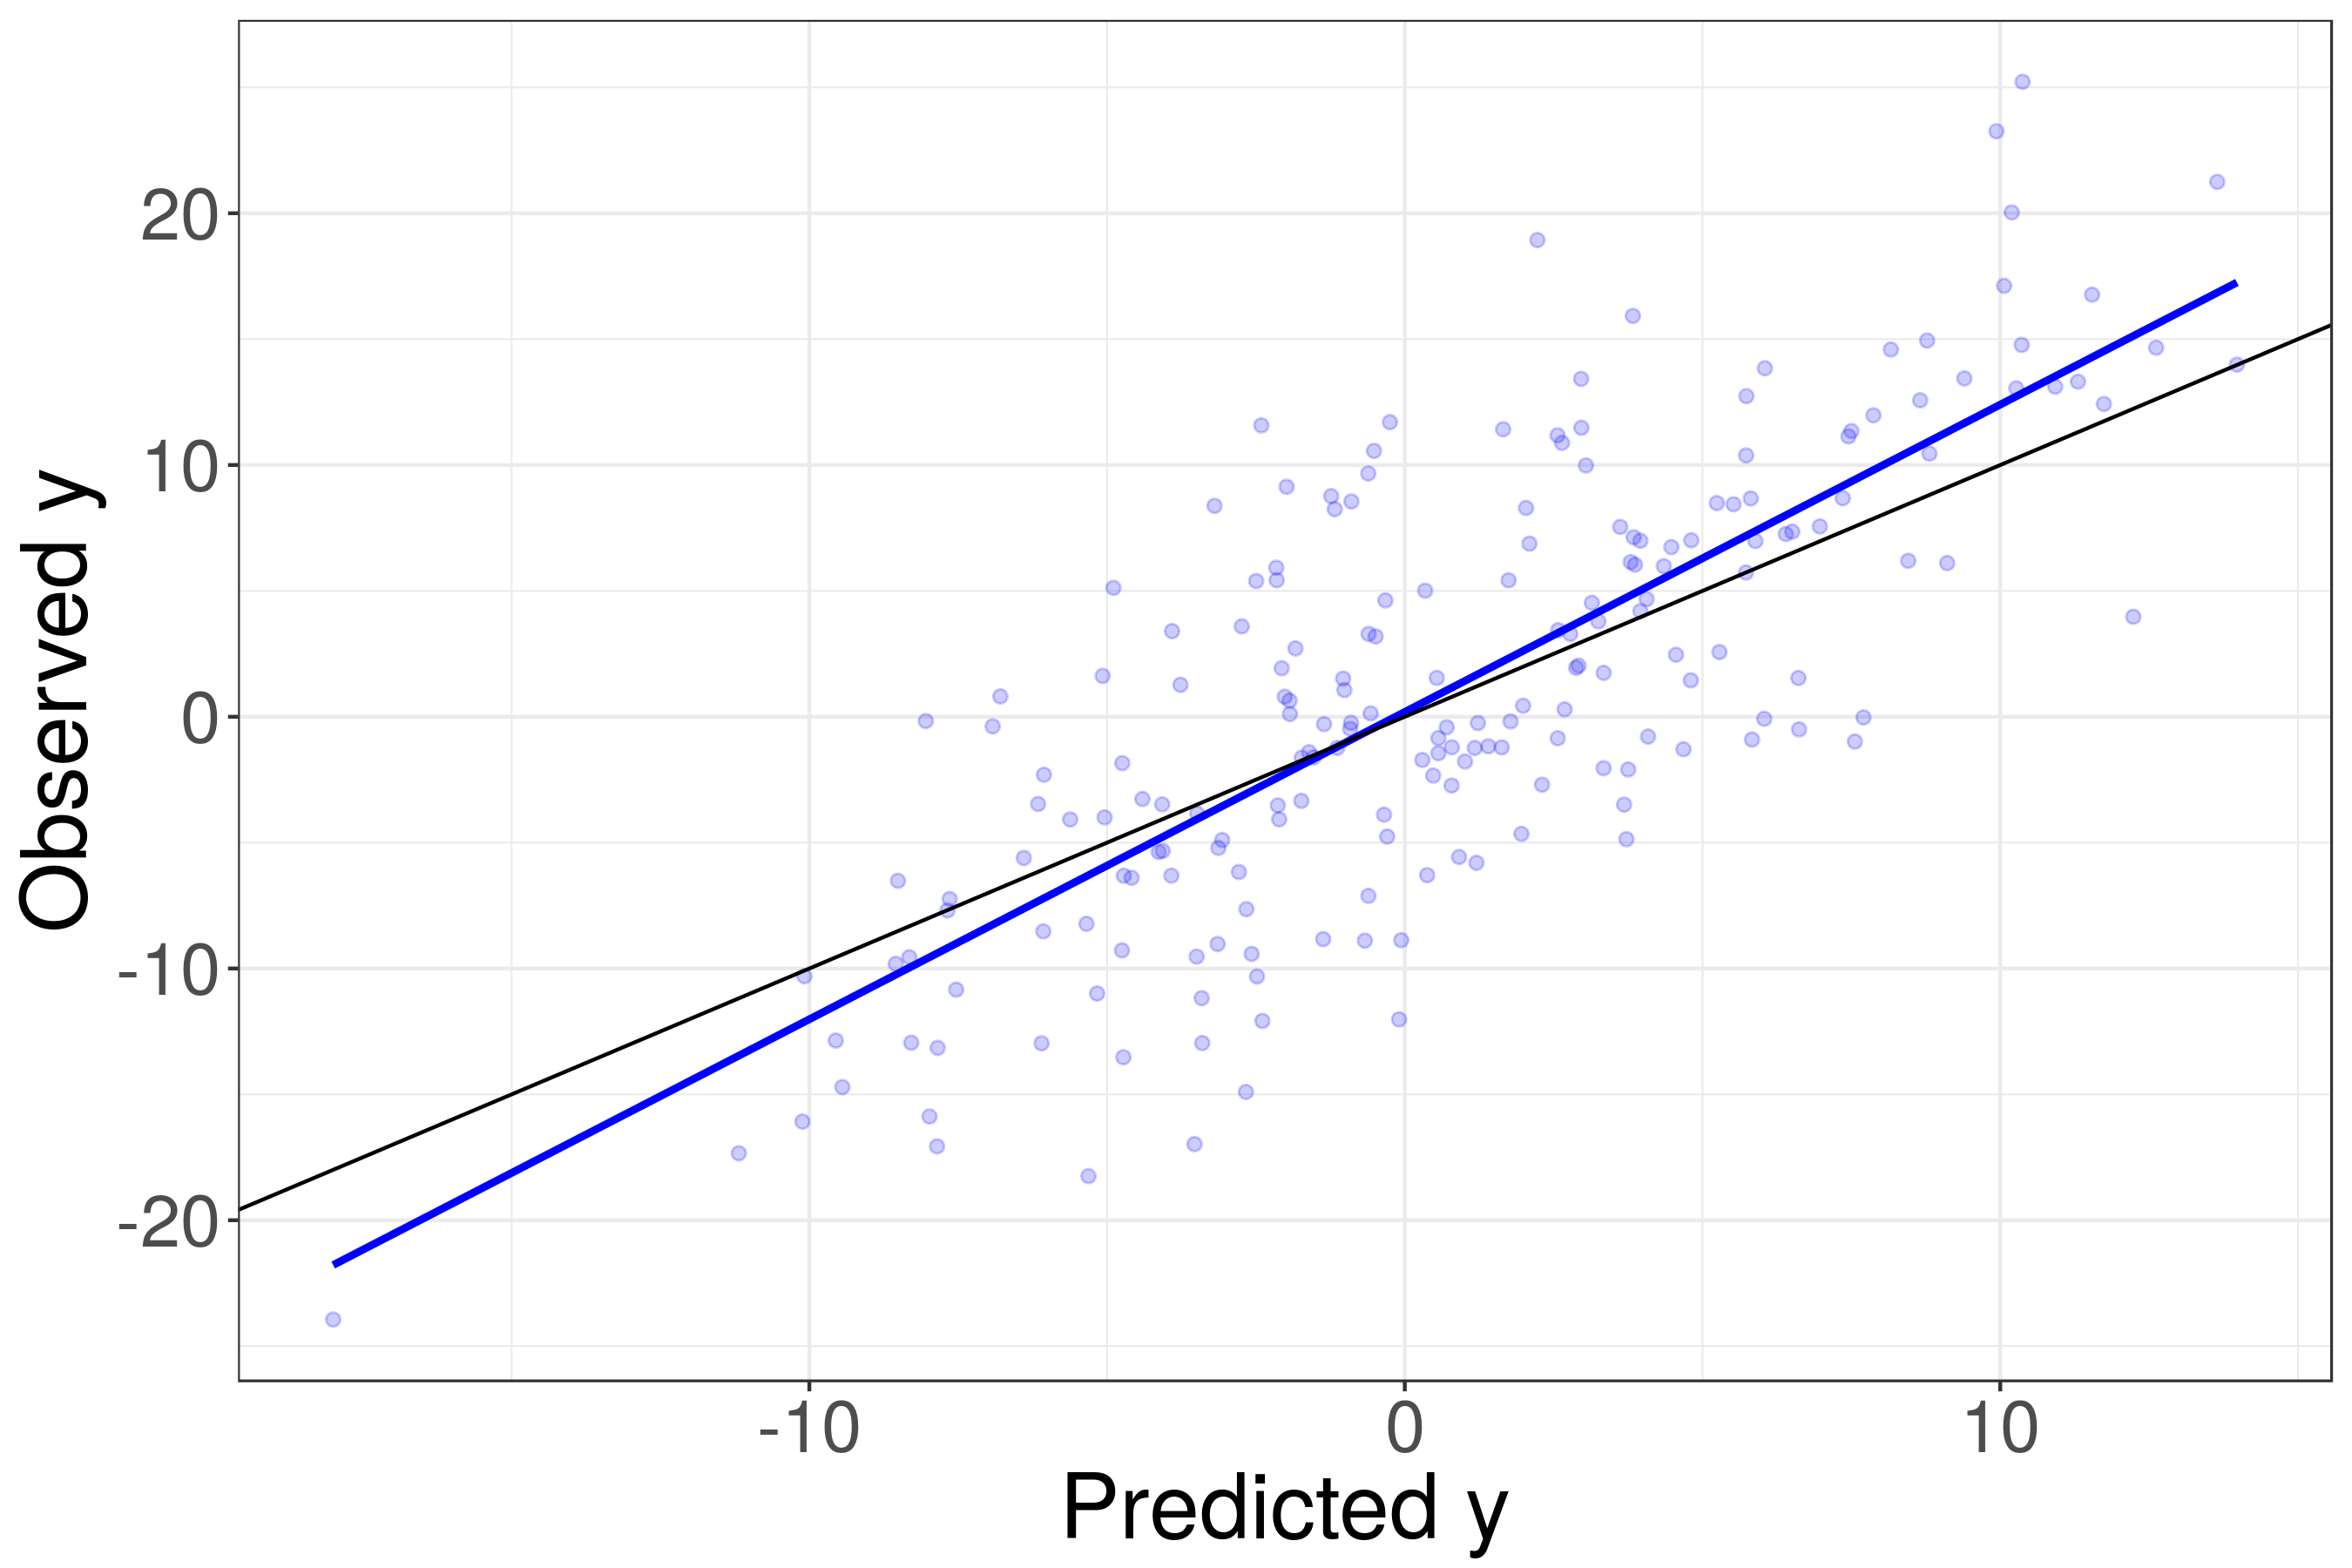
\includegraphics[width = \textwidth]{./lasso_figures/obs_y_vs_pred2.png}
  \end{subfigure}
  \caption{(a) Log(slope) of $y$ on $\hat y = x^T\hat\beta^{lasso}_\lambda$ as a function of $\log(\lambda)$.
	Vertical red line is the $\lambda$
  chosen by cross-validation. Yellow are slopes in the training sample, blue is slope in the test sample.
  (b) Scatterplot of $(y_{new}, \hat y)$ in the test sample, where
	$\hat y$ computed with the LASSO objective with the same $\lambda$ chosen by cross-validation in (a), and
	the blue line is the regression line.
	Black line is the 45 degree line. }
	\label{fig:lasso_results_fixed}
\end{figure}

\noindent{\bf Varying noise} \par
We investigate if this is a consistent occurrence by repeating this experiment 500 times. Moreover, we see if varying the
noise parameter $\sigma$ has any effect. In total, we run this experiment 500 times for each value of $\sigma$, and our results are
displayed in figure \ref{fig:lasso_results_vary_sigma}. Figure \ref{fig:lasso_results_vary_sigma}a shows the median slope across
500 trials for varying $\sigma$. We see that choosing $\lambda$ and $K$ either jointly or in two steps results in smaller median
slope,
for all $\sigma$. However, for small $\sigma$, choosing $K$ results in a median slope less than 1,
and we have over-compensated. Figure
\ref{fig:lasso_results_vary_sigma}b displays the relative test set MSPE of choosing $\lambda$ and $K$ over
the MSPE to choosing just $\lambda$. It does not seem that choosing $K$ in addition to $\lambda$ improves MSPE,
and it does worse when $\sigma$ is small.

In all cases, running LASSO for feature selection and then applying the Copas procedure to the selected features gave the
worst results. This perhaps is unsurprising given that LASSO was unable to recover the true non-zero coefficients, so the
Copas procedure did not work well.

\begin{figure}[!h]
	\centering
	\begin{subfigure}[t]{0.45\textwidth}
		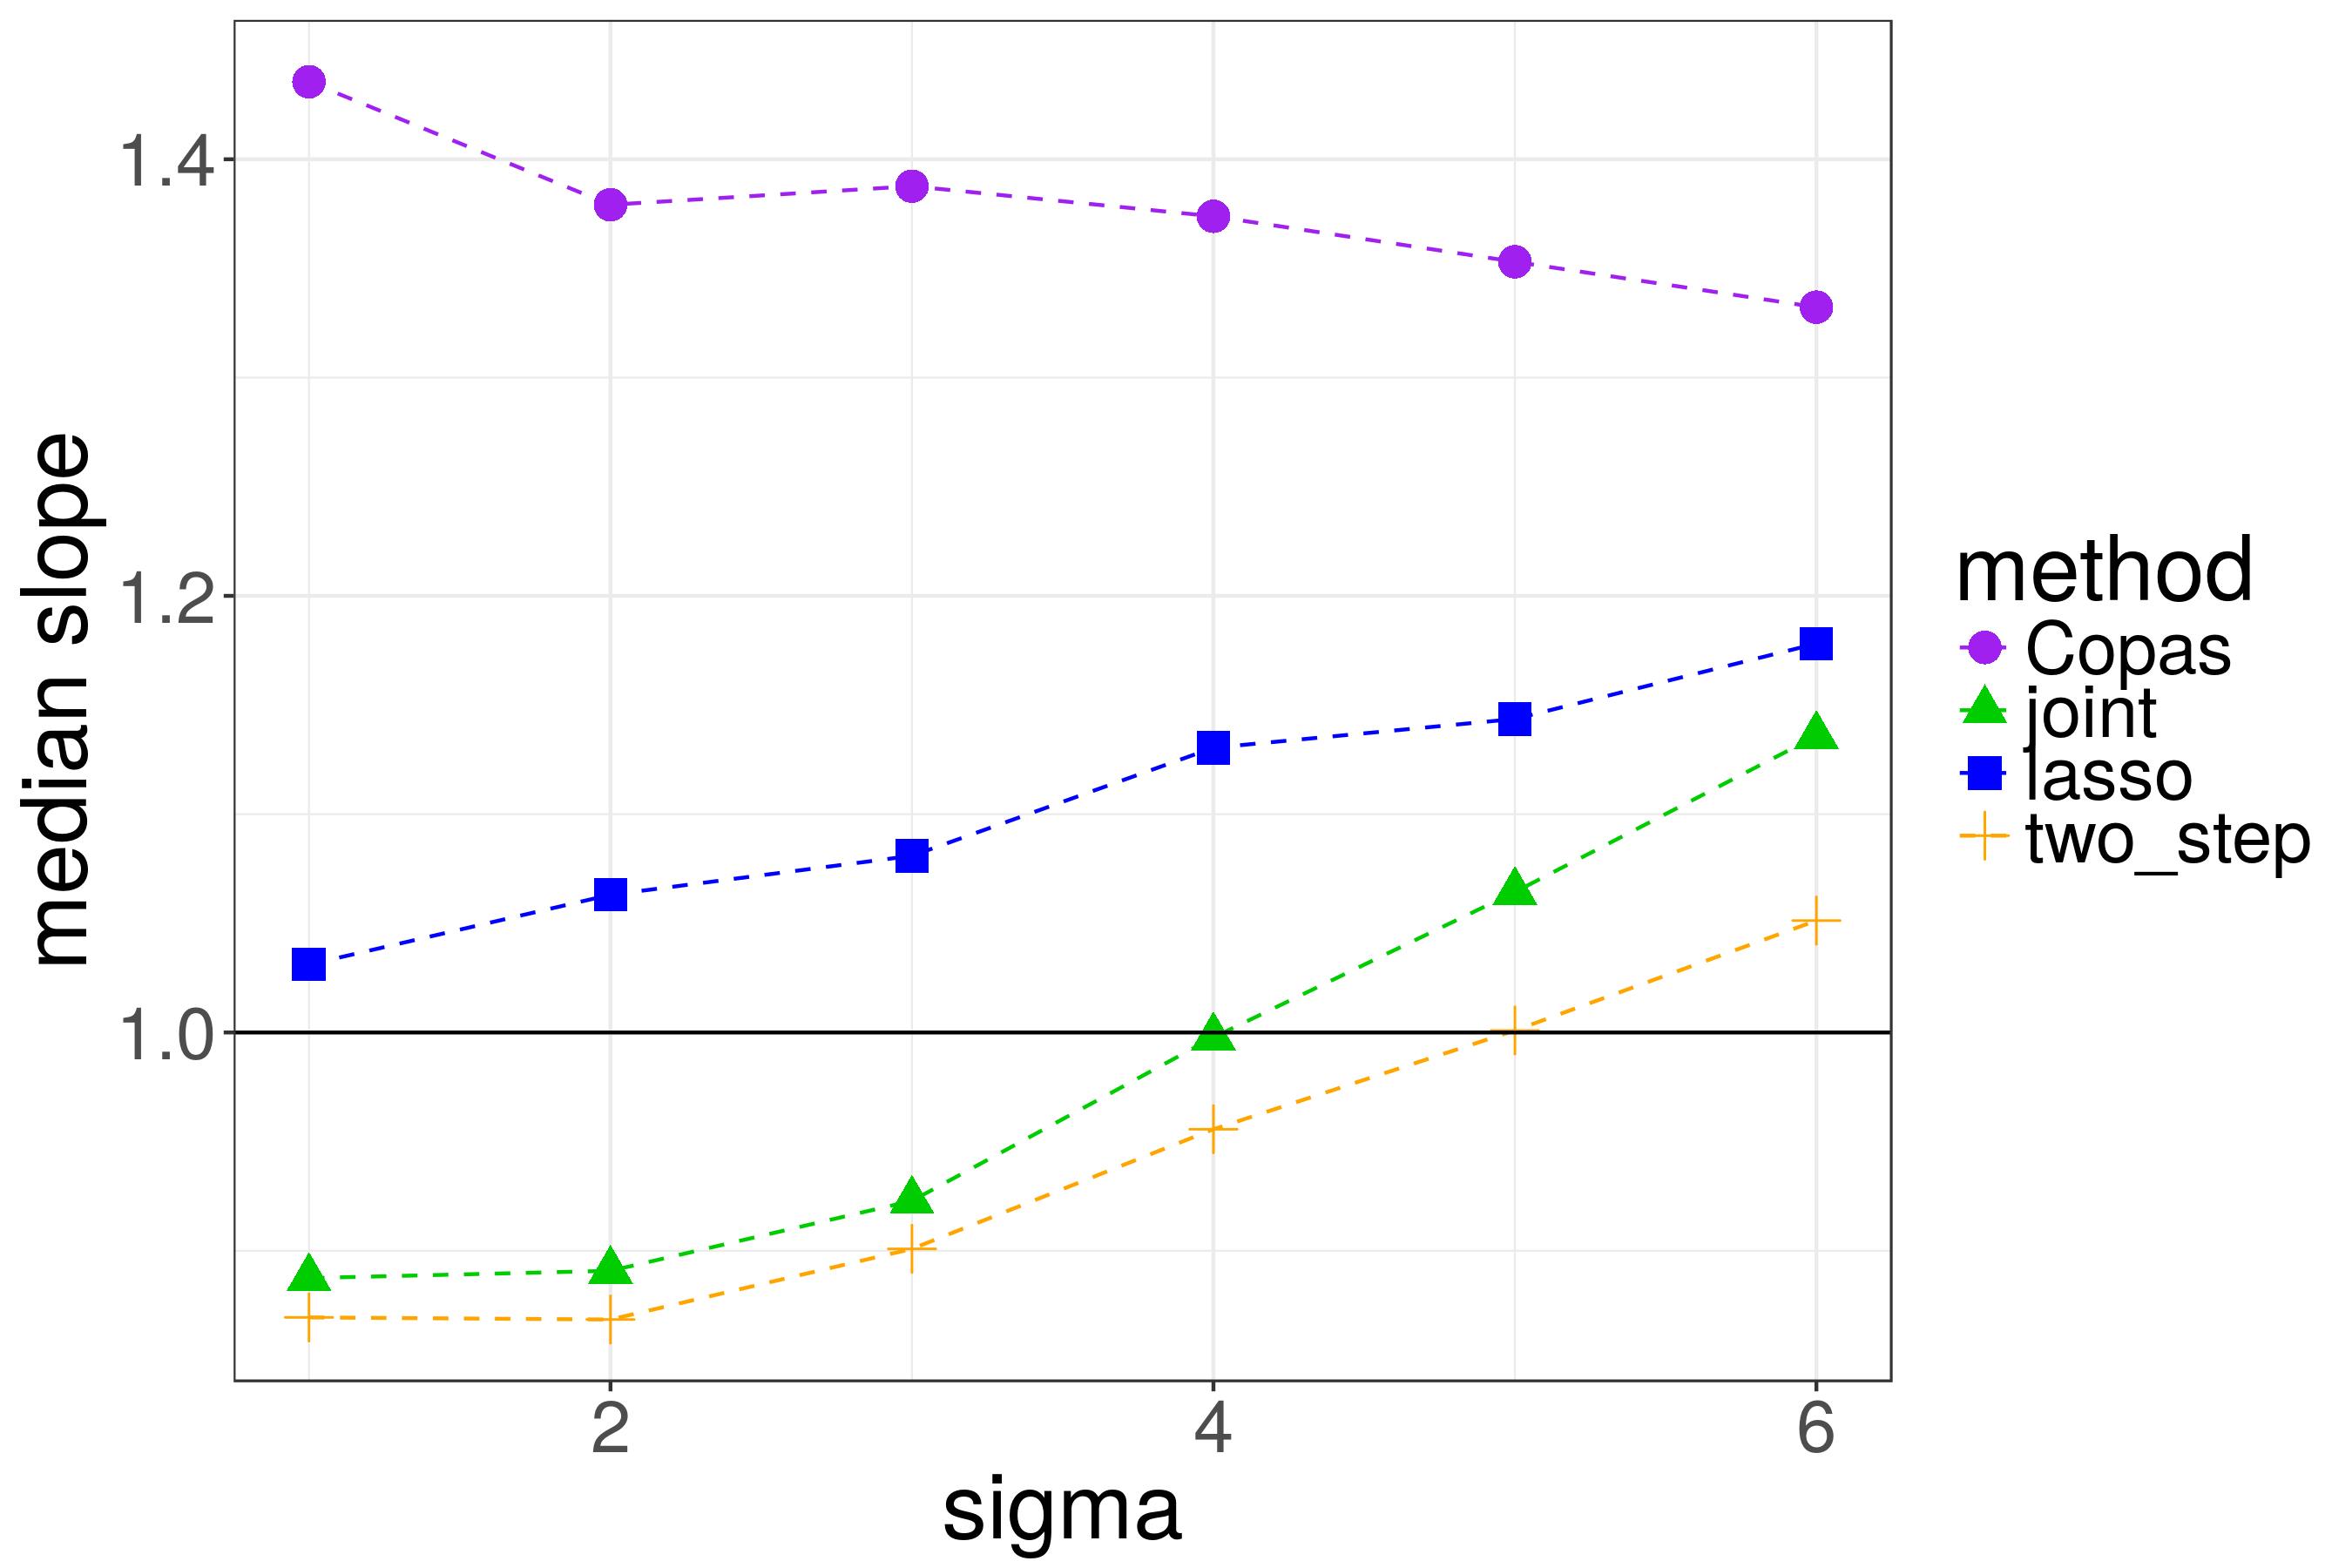
\includegraphics[width = \textwidth]{./lasso_figures/slope_vs_sigma.png}
	\end{subfigure}
  \begin{subfigure}[t]{0.45\textwidth}
    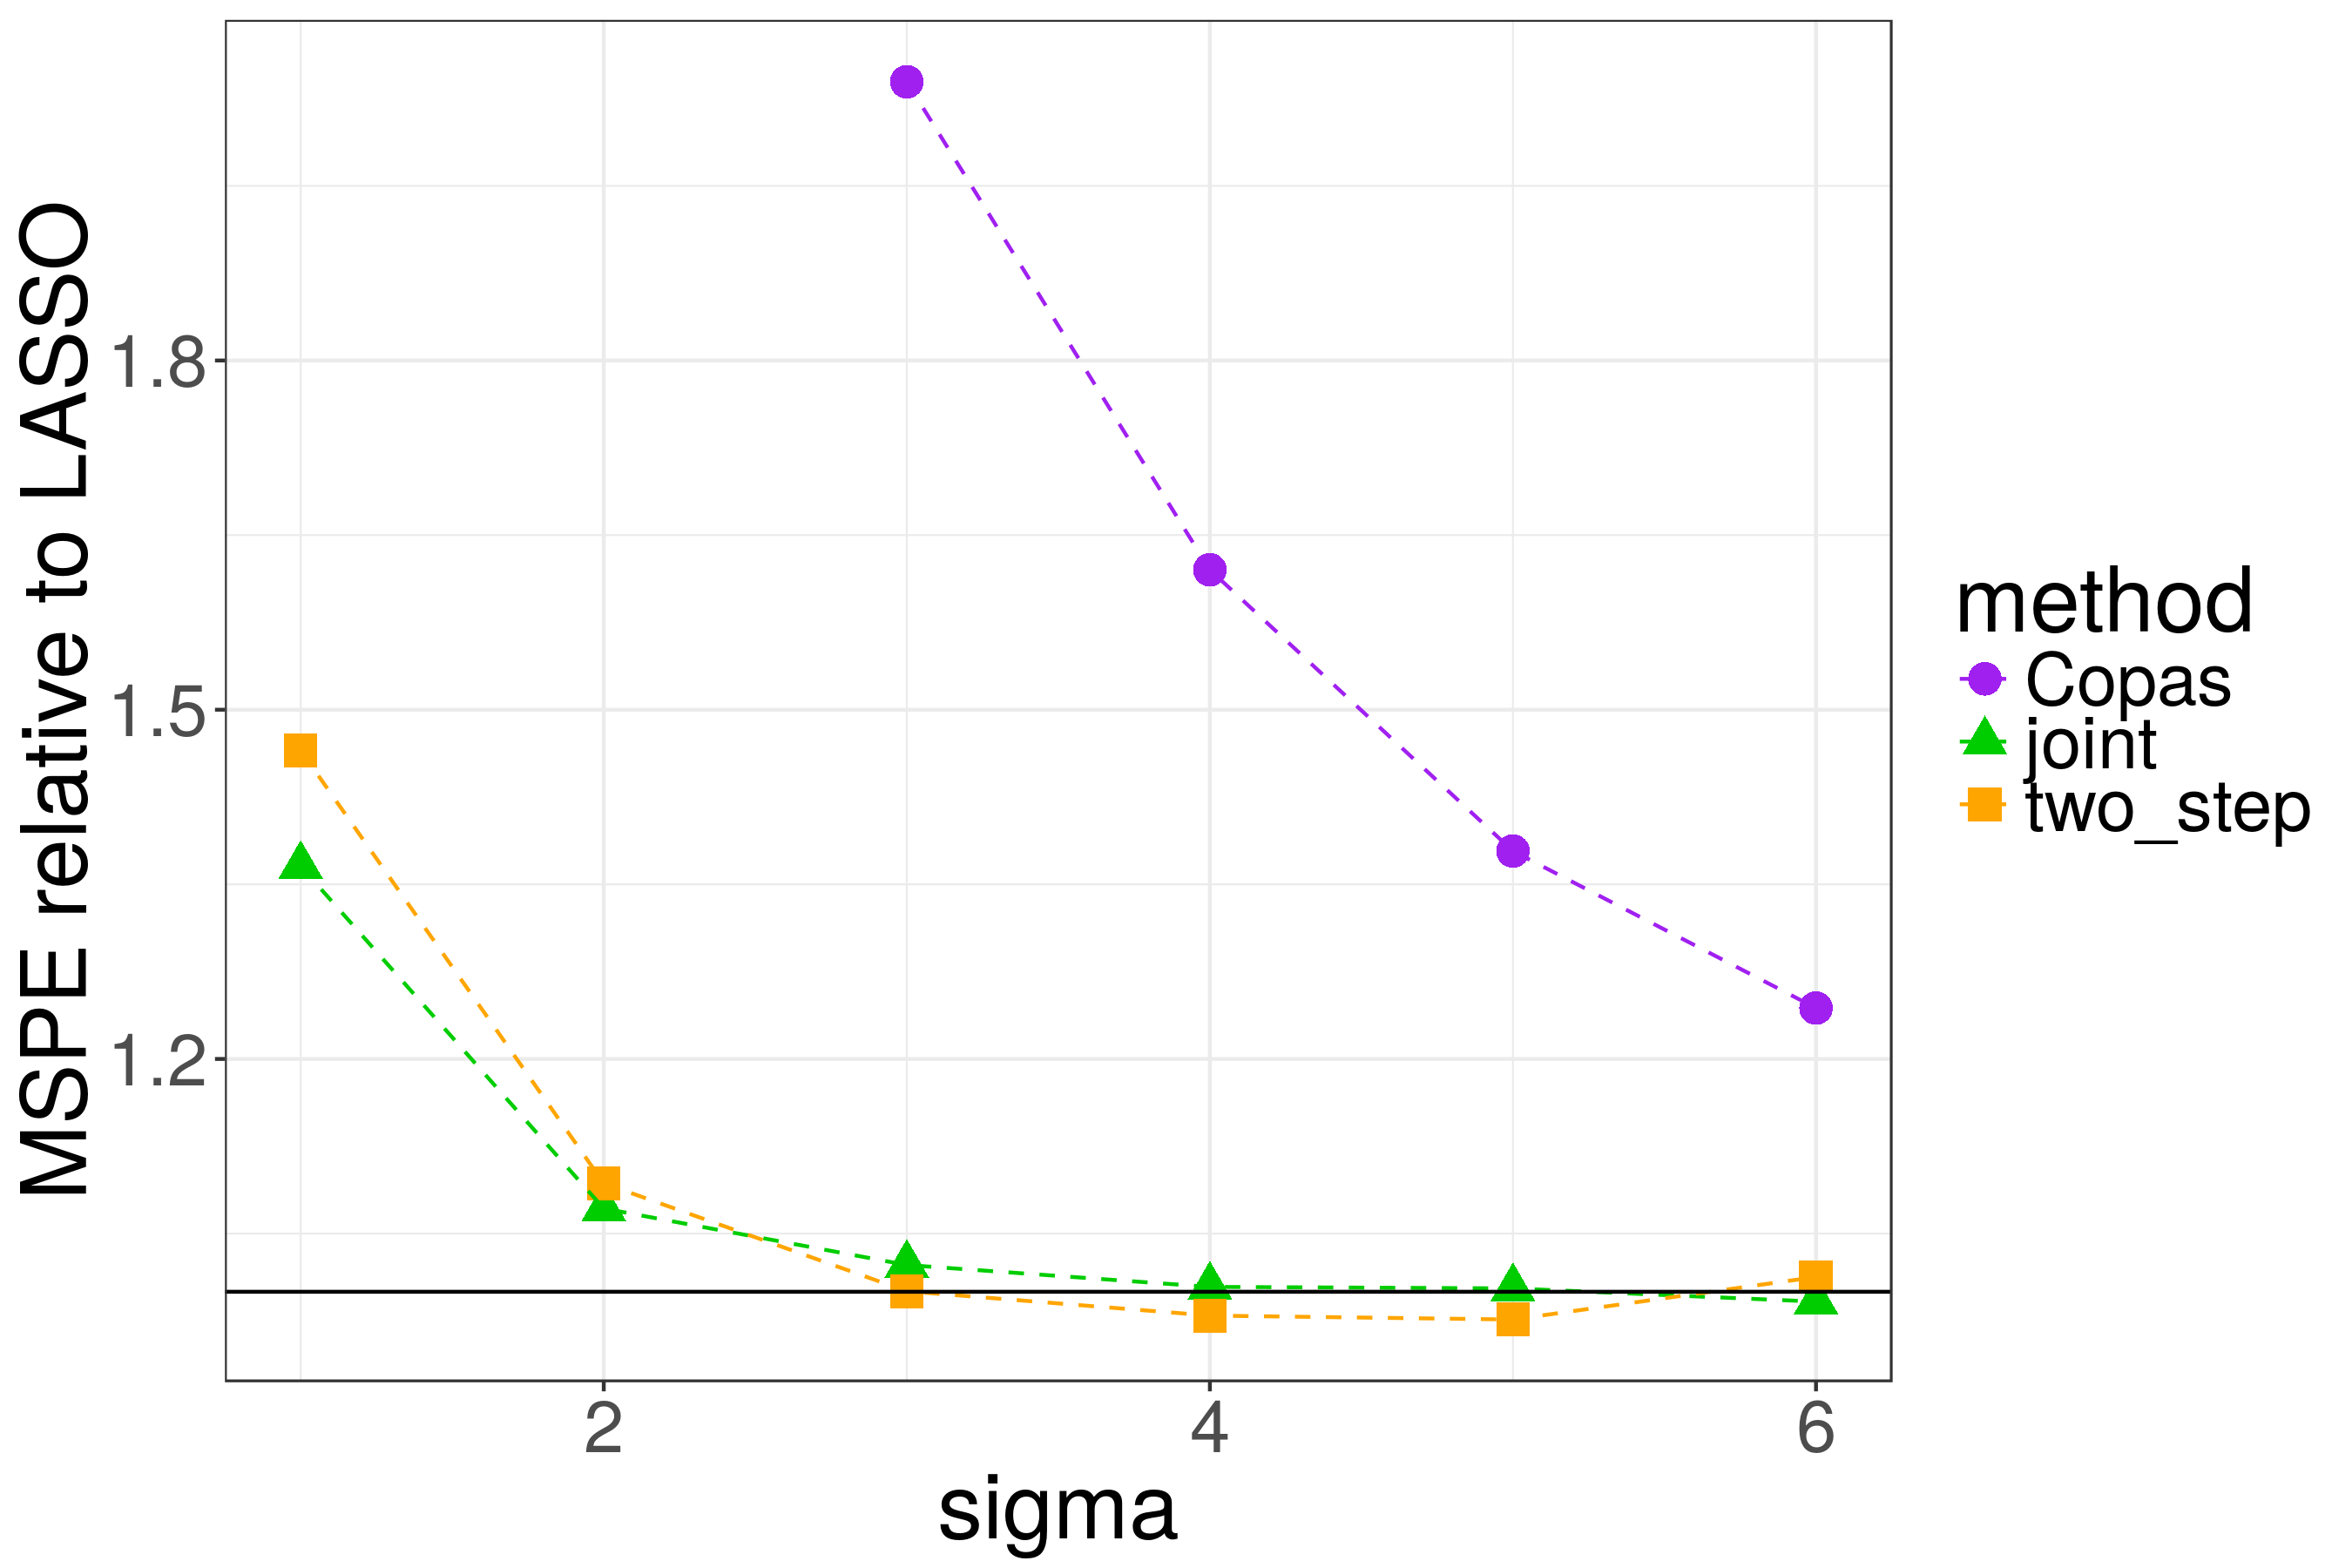
\includegraphics[width = \textwidth]{./lasso_figures/mspe_vs_sigma.png}
  \end{subfigure}
  \caption{(a) Median $\text{slope}(y_{new}, \hat y)$ over 500 trials, as a function of the noise $\sigma$. (b)
	The median relative test set MSPEs to the
	traditional LASSO procedure, as a function of the noise $\sigma$. }
	\label{fig:lasso_results_vary_sigma}
\end{figure}

\noindent{\bf Varying sparsity} \par
Next, we examine the performance of our procedure relative to the traditional LASSO procedure as the sparsity varies. In figure
\ref{fig:lasso_results_vary_sparsity}a, we again compare the slopes; in figure \ref{fig:lasso_results_vary_sparsity}b, we
compare the MSPEs. It appears that selecting $K$ either jointly or in two stages with $\lambda$ does not yield significant improvements in MSPE
for the sparsity levels we examined. Running LASSO for feature selection and then applying the Copas procedure again
did the worst, and its performance is particularly bad when the number of non-zero coefficients gets larger.

\begin{figure}[!h]
	\centering
	\begin{subfigure}[t]{0.45\textwidth}
		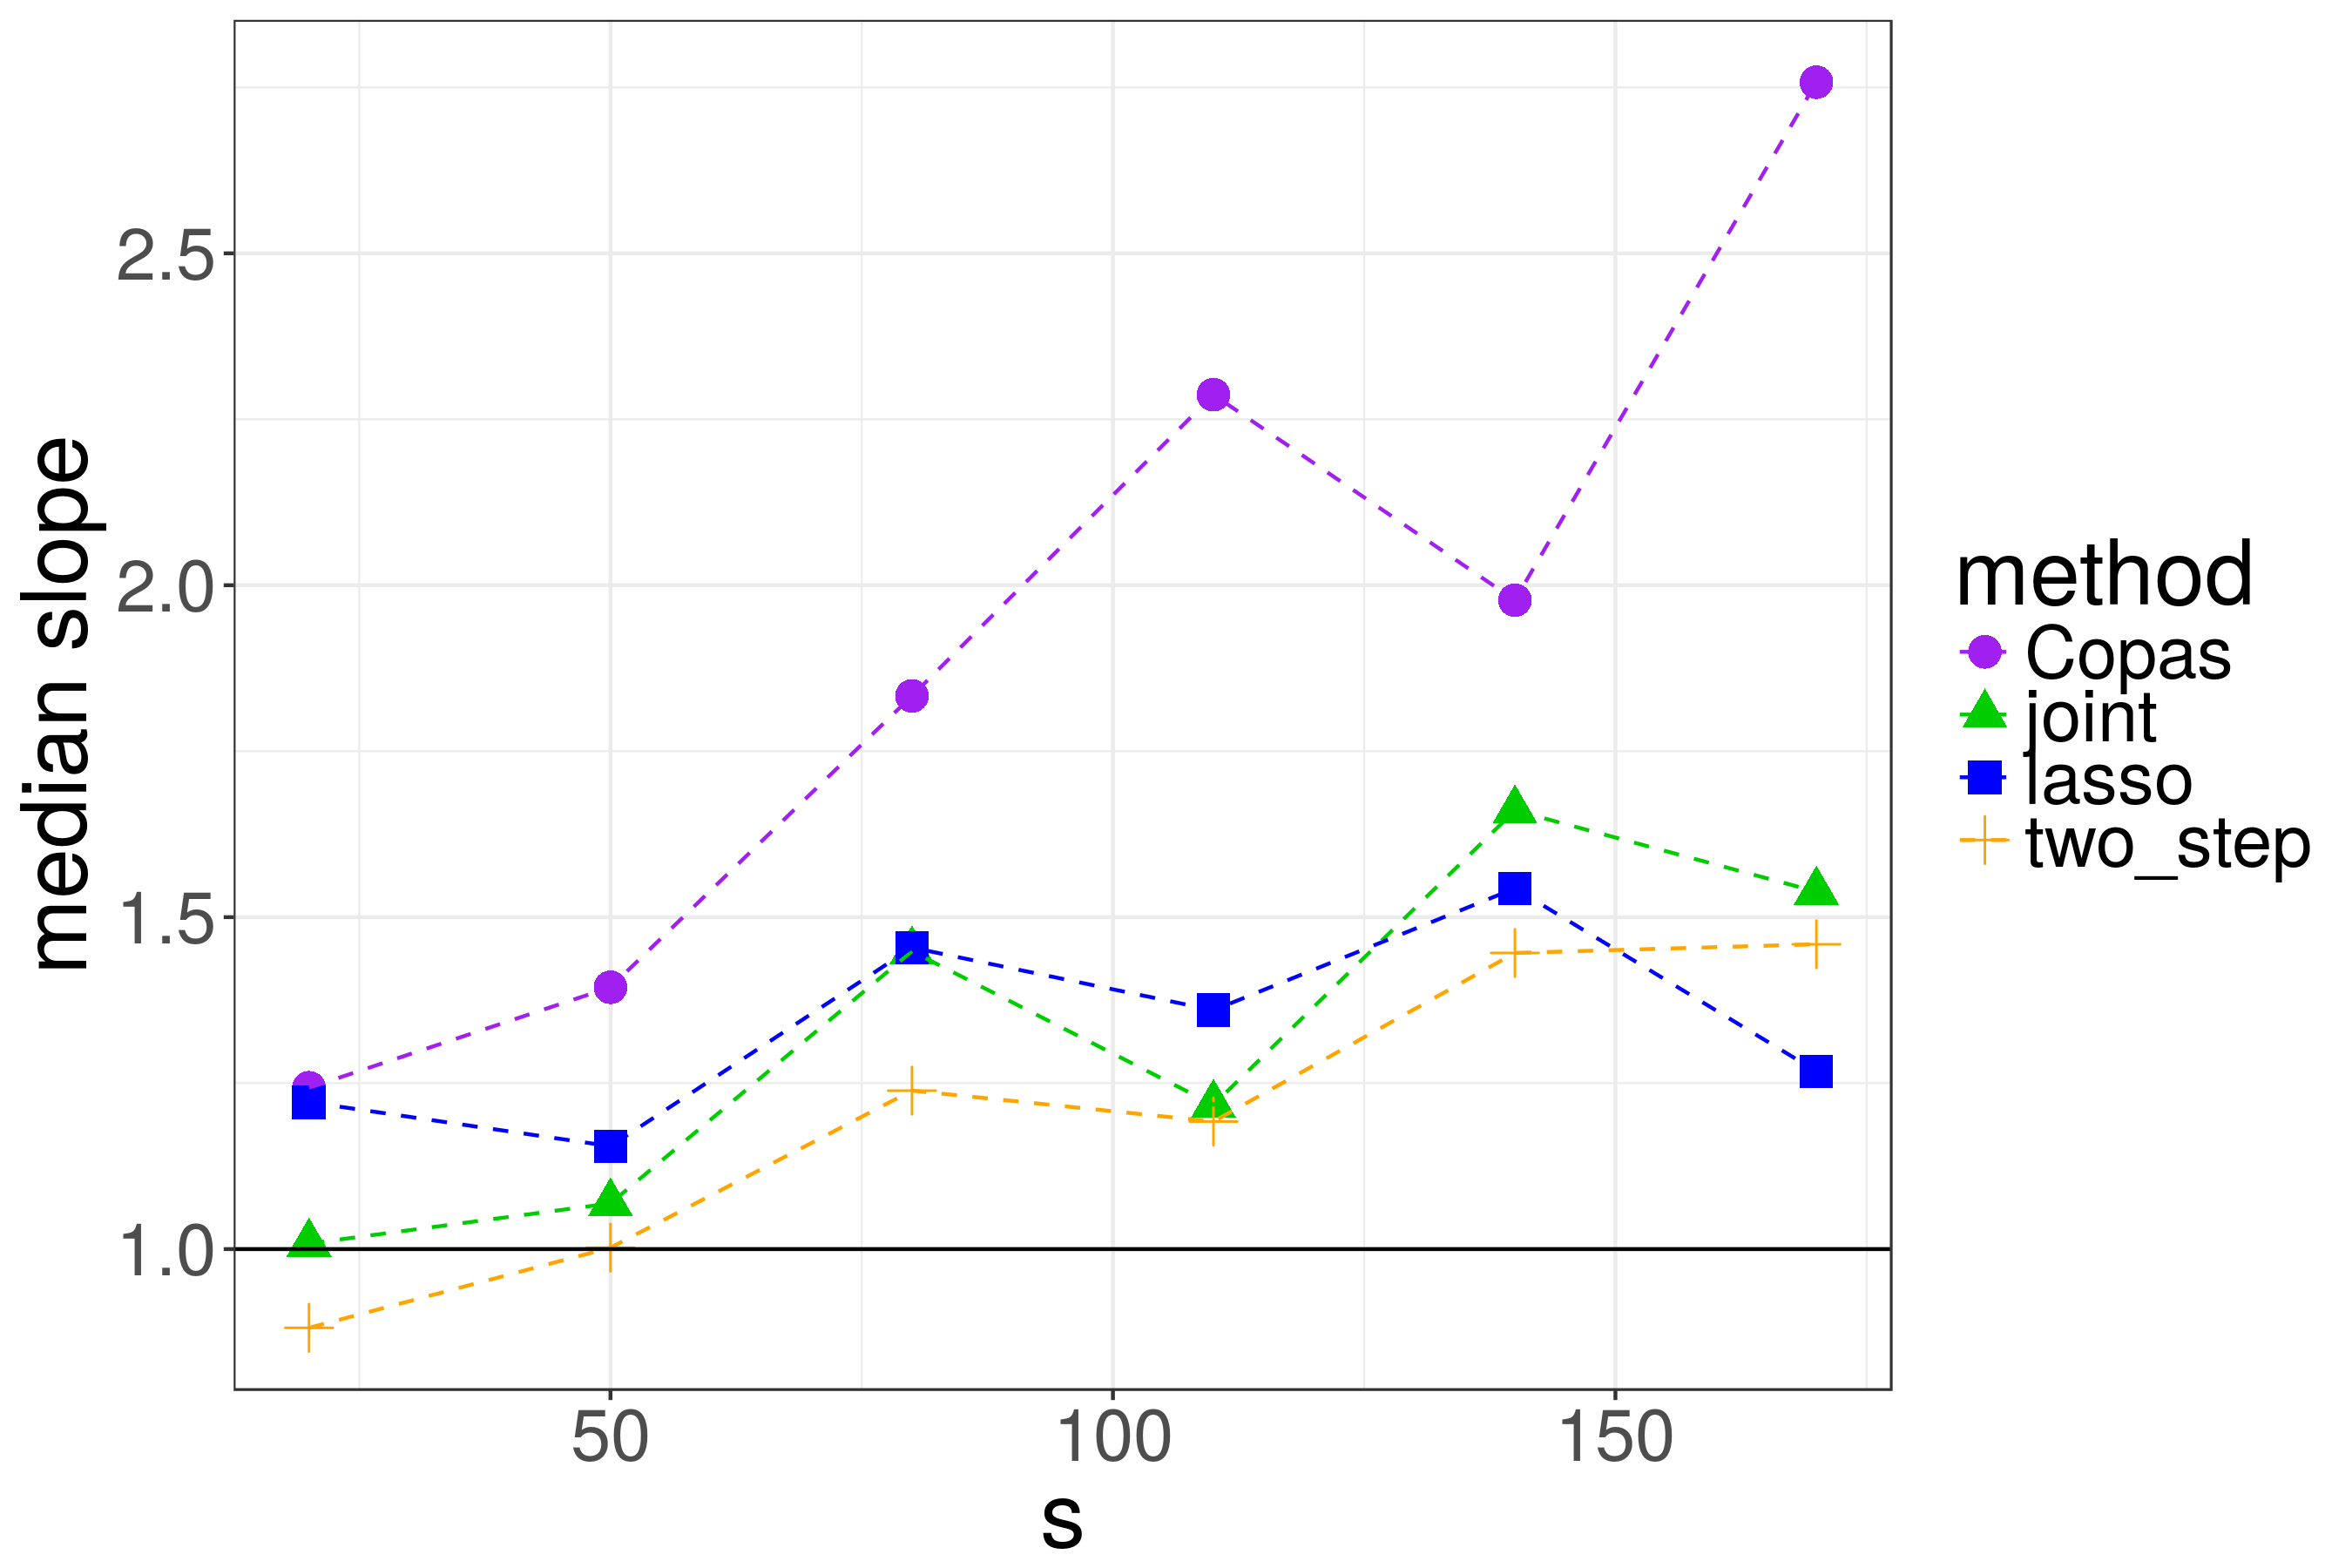
\includegraphics[width = \textwidth]{./lasso_figures/slope_vs_sparsity.png}
	\end{subfigure}
  \begin{subfigure}[t]{0.45\textwidth}
    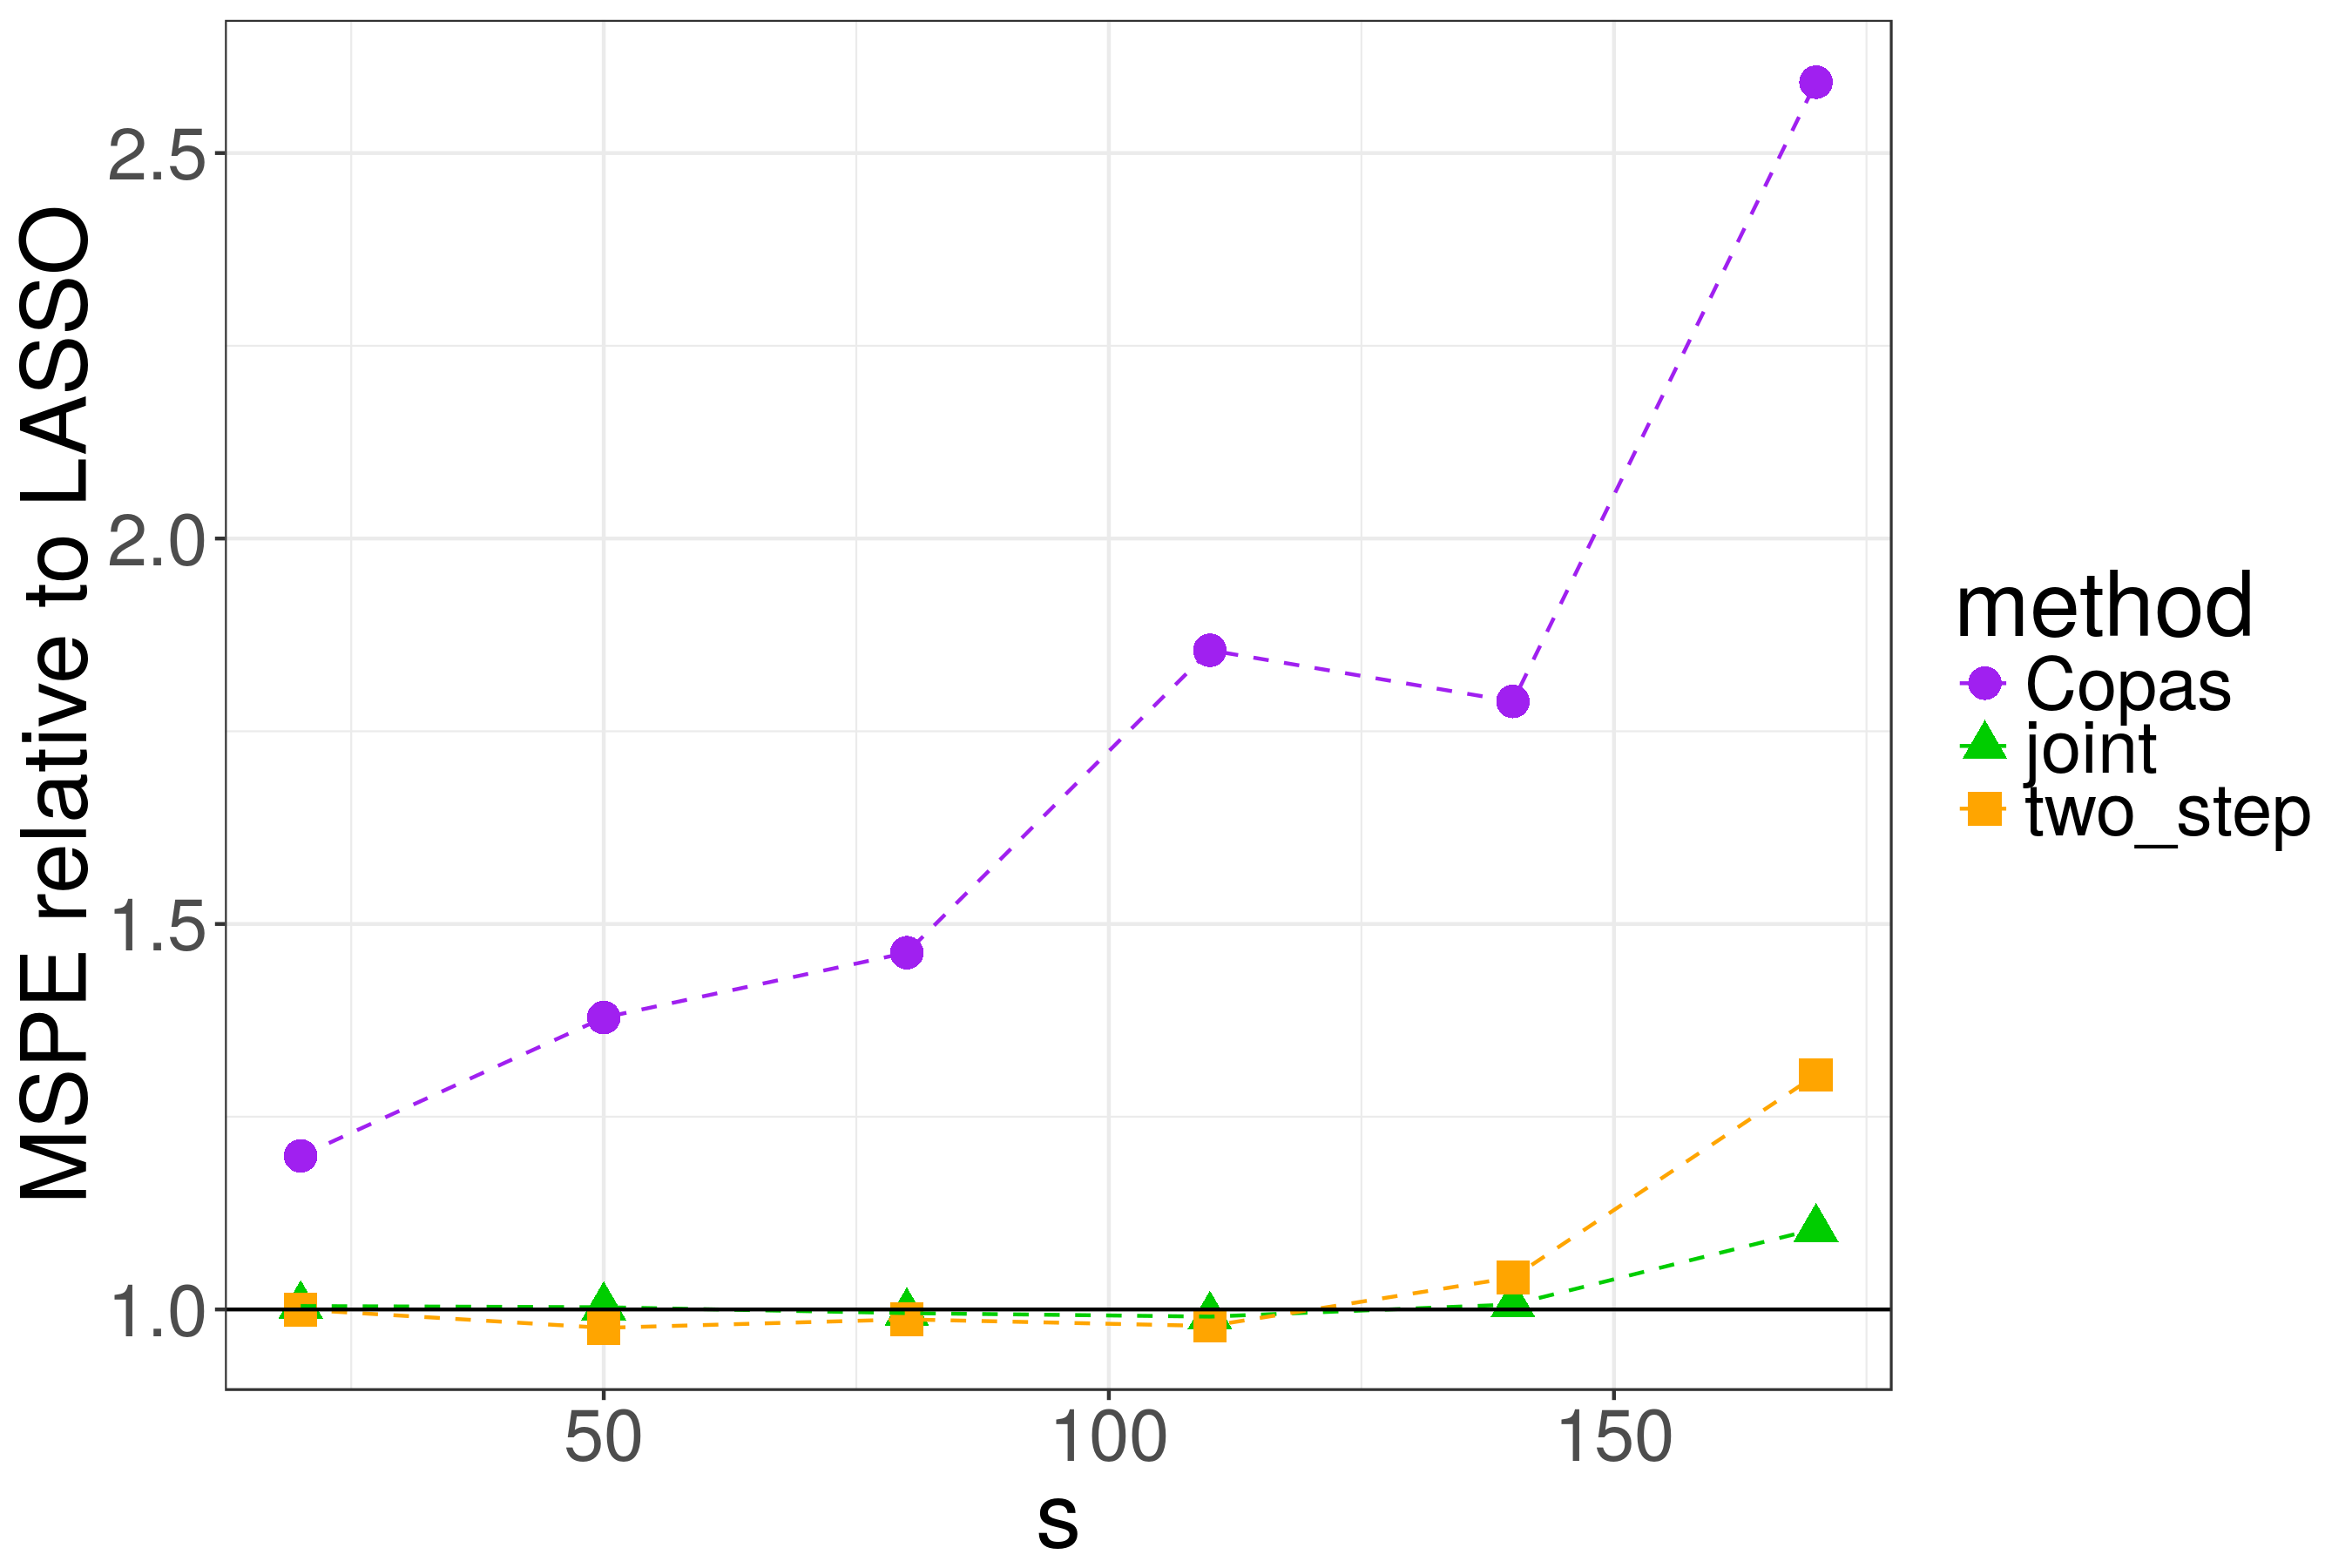
\includegraphics[width = \textwidth]{./lasso_figures/mspe_vs_sparsity.png}
  \end{subfigure}
  \caption{(a) Median $\text{slope}(y_{new}, \hat y)$ over 500 trials, as a function of number of nonzero coefficients $s$.
	(b)
	The median relative MSPEs of our method to the
	traditional LASSO procedure, as a function of the noise $\sigma$.  }
	\label{fig:lasso_results_vary_sparsity}
\end{figure}

\subsection{Single-response analysis of fMRI data}

For each of the twenty voxels, we predict its response to the image a subject was viewing at the time.
Features were extracted from an
image using a Gabor wavelet tranformation, resulting in $p = 10921$ features.
We used $n = 1225$ observations in our training set, and held out $N = 525$ observations in our test set. We predict the response
first using LASSO, where $\lambda$ was selected using cross-validation on the training set. We compare this performance with
using LASSO but where we select $K$ jointly with $\lambda$ (again using cross-validation on the training set).

The results are shown in figure \ref{fig:fmri_single_response_results}, which display the slopes and MSPEs on the test set.
We see that for 13 of the 20 voxels, choosing $K$ jointly with $\lambda$ resulted in slopes closer to 1; there are some voxels,
like voxel 16, where our method gave a slope further from one.  MSPEs for both methods in all the voxels however,
were rather similar.

\begin{figure}[!h]
	\centering
	\begin{subfigure}[t]{0.45\textwidth}
		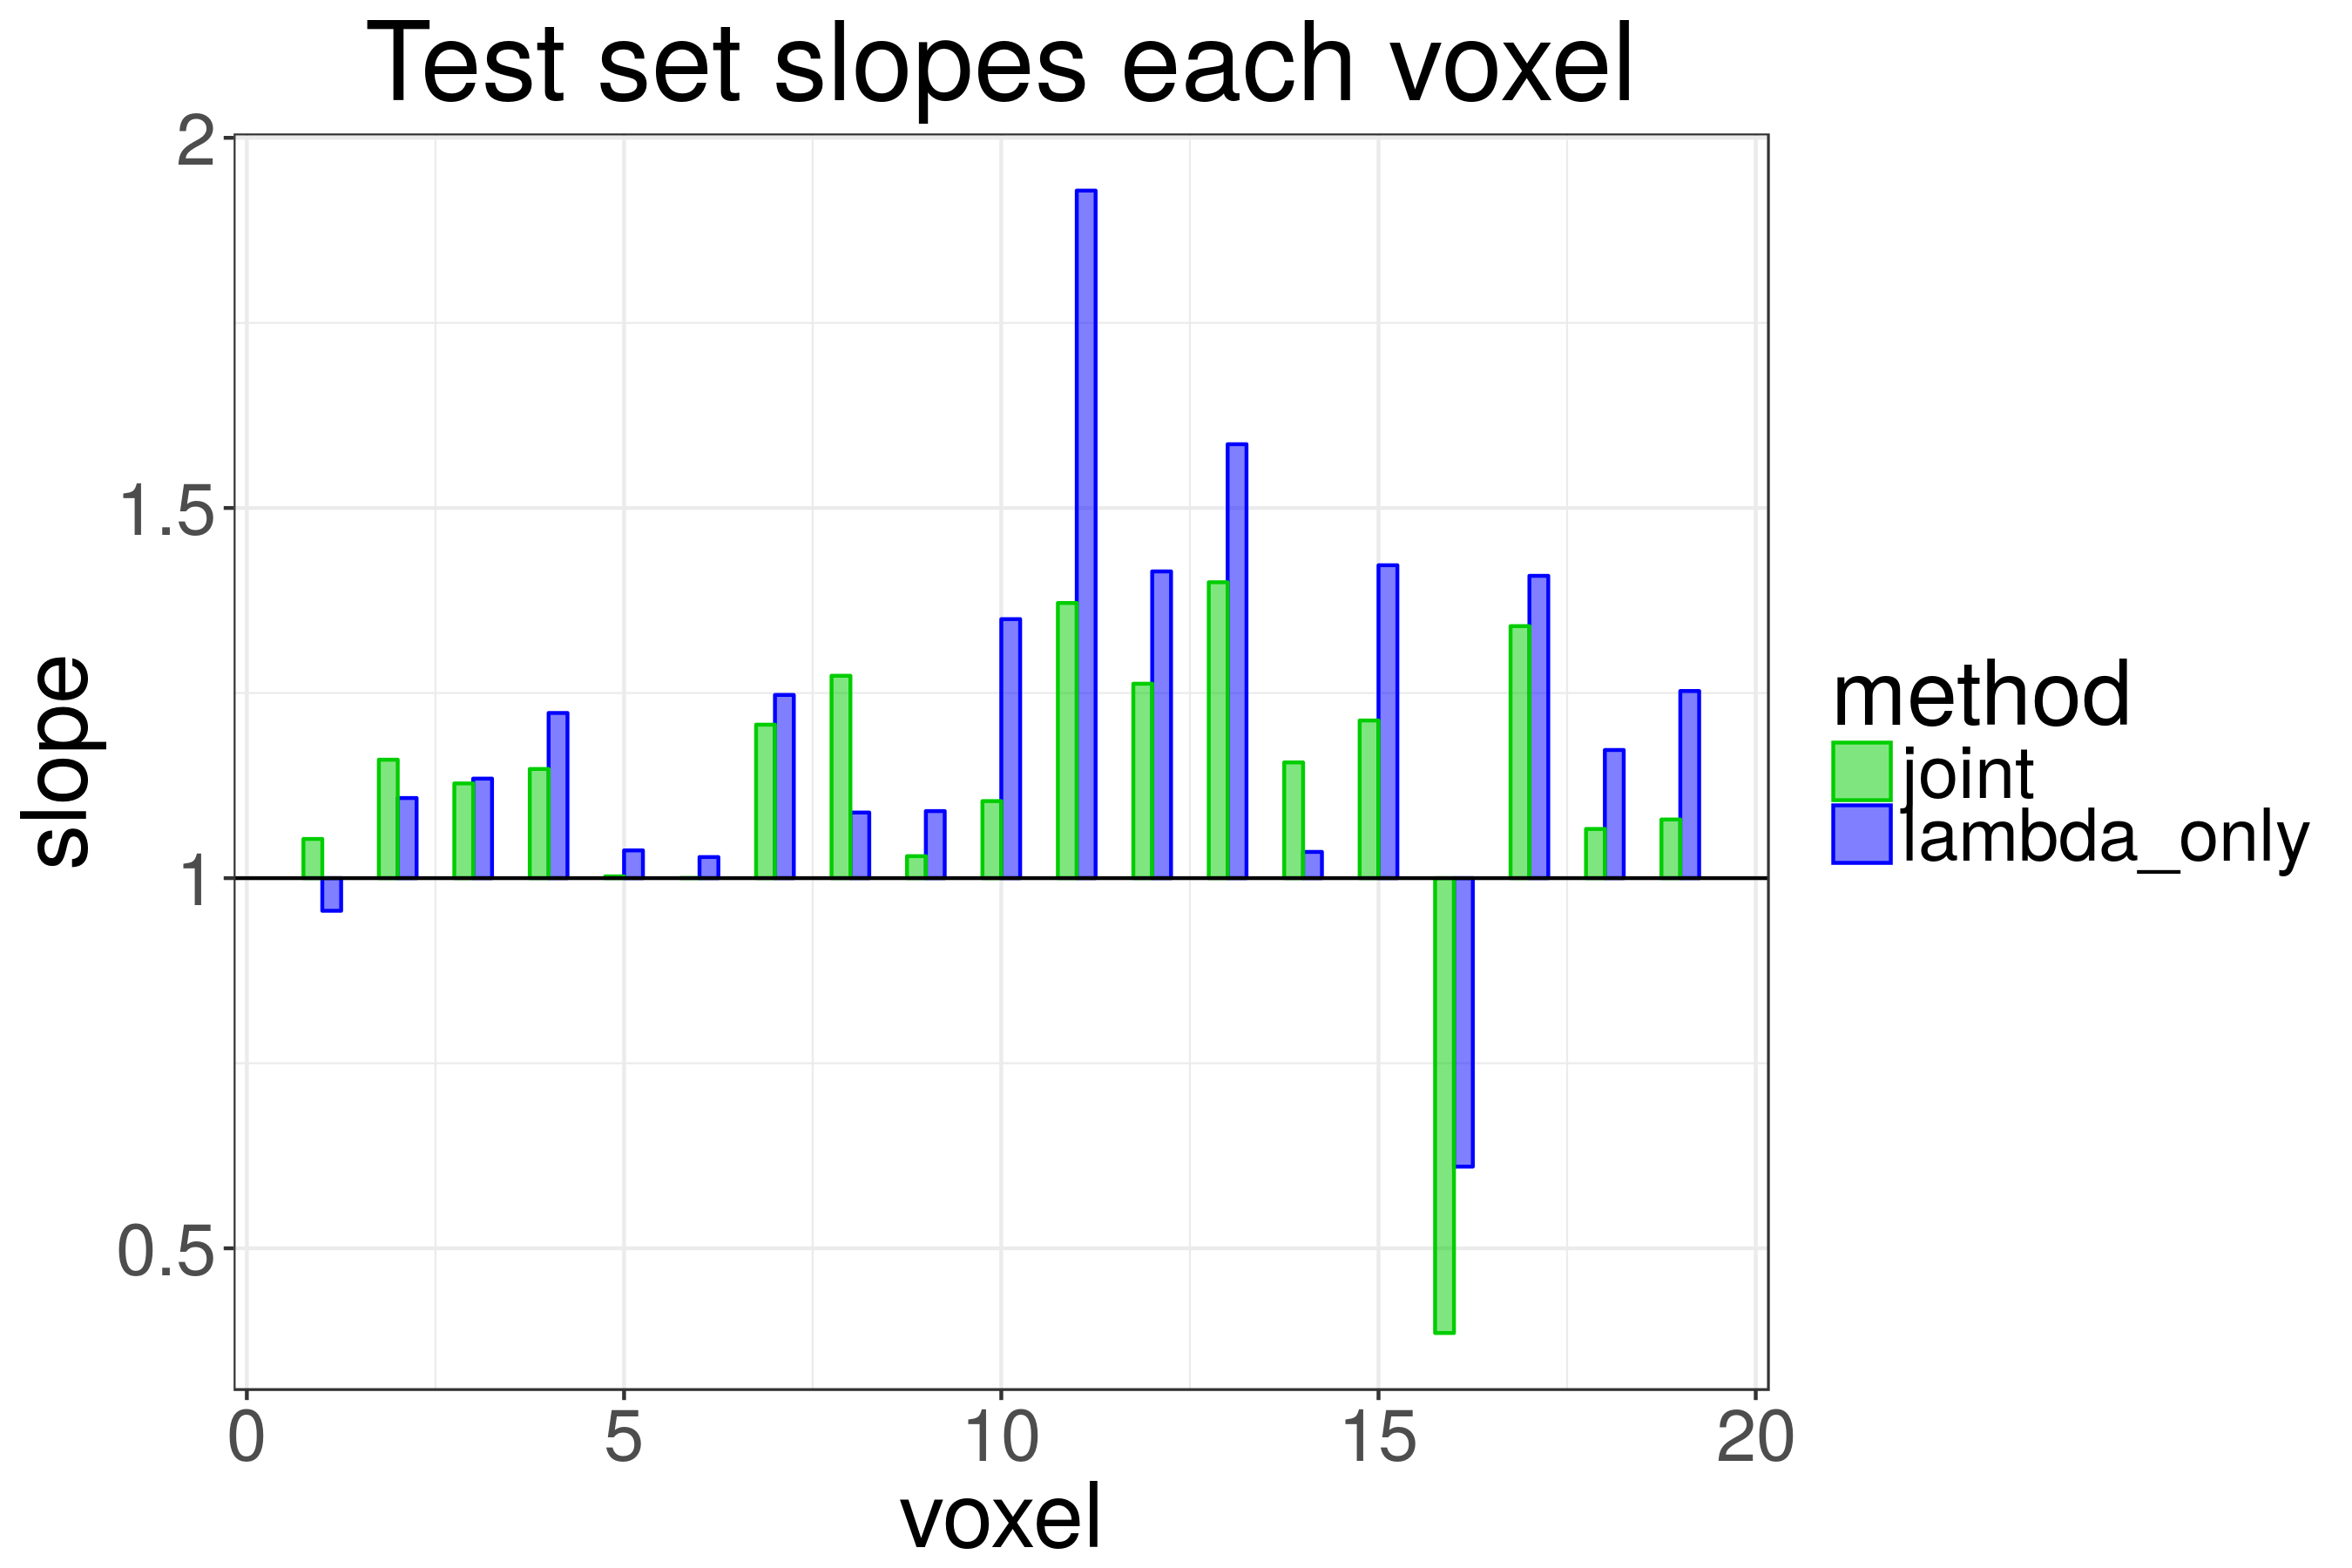
\includegraphics[width = \textwidth]{./single_response_fmri_figures/fmri_slopes.png}
	\end{subfigure}
	\begin{subfigure}[t]{0.45\textwidth}
		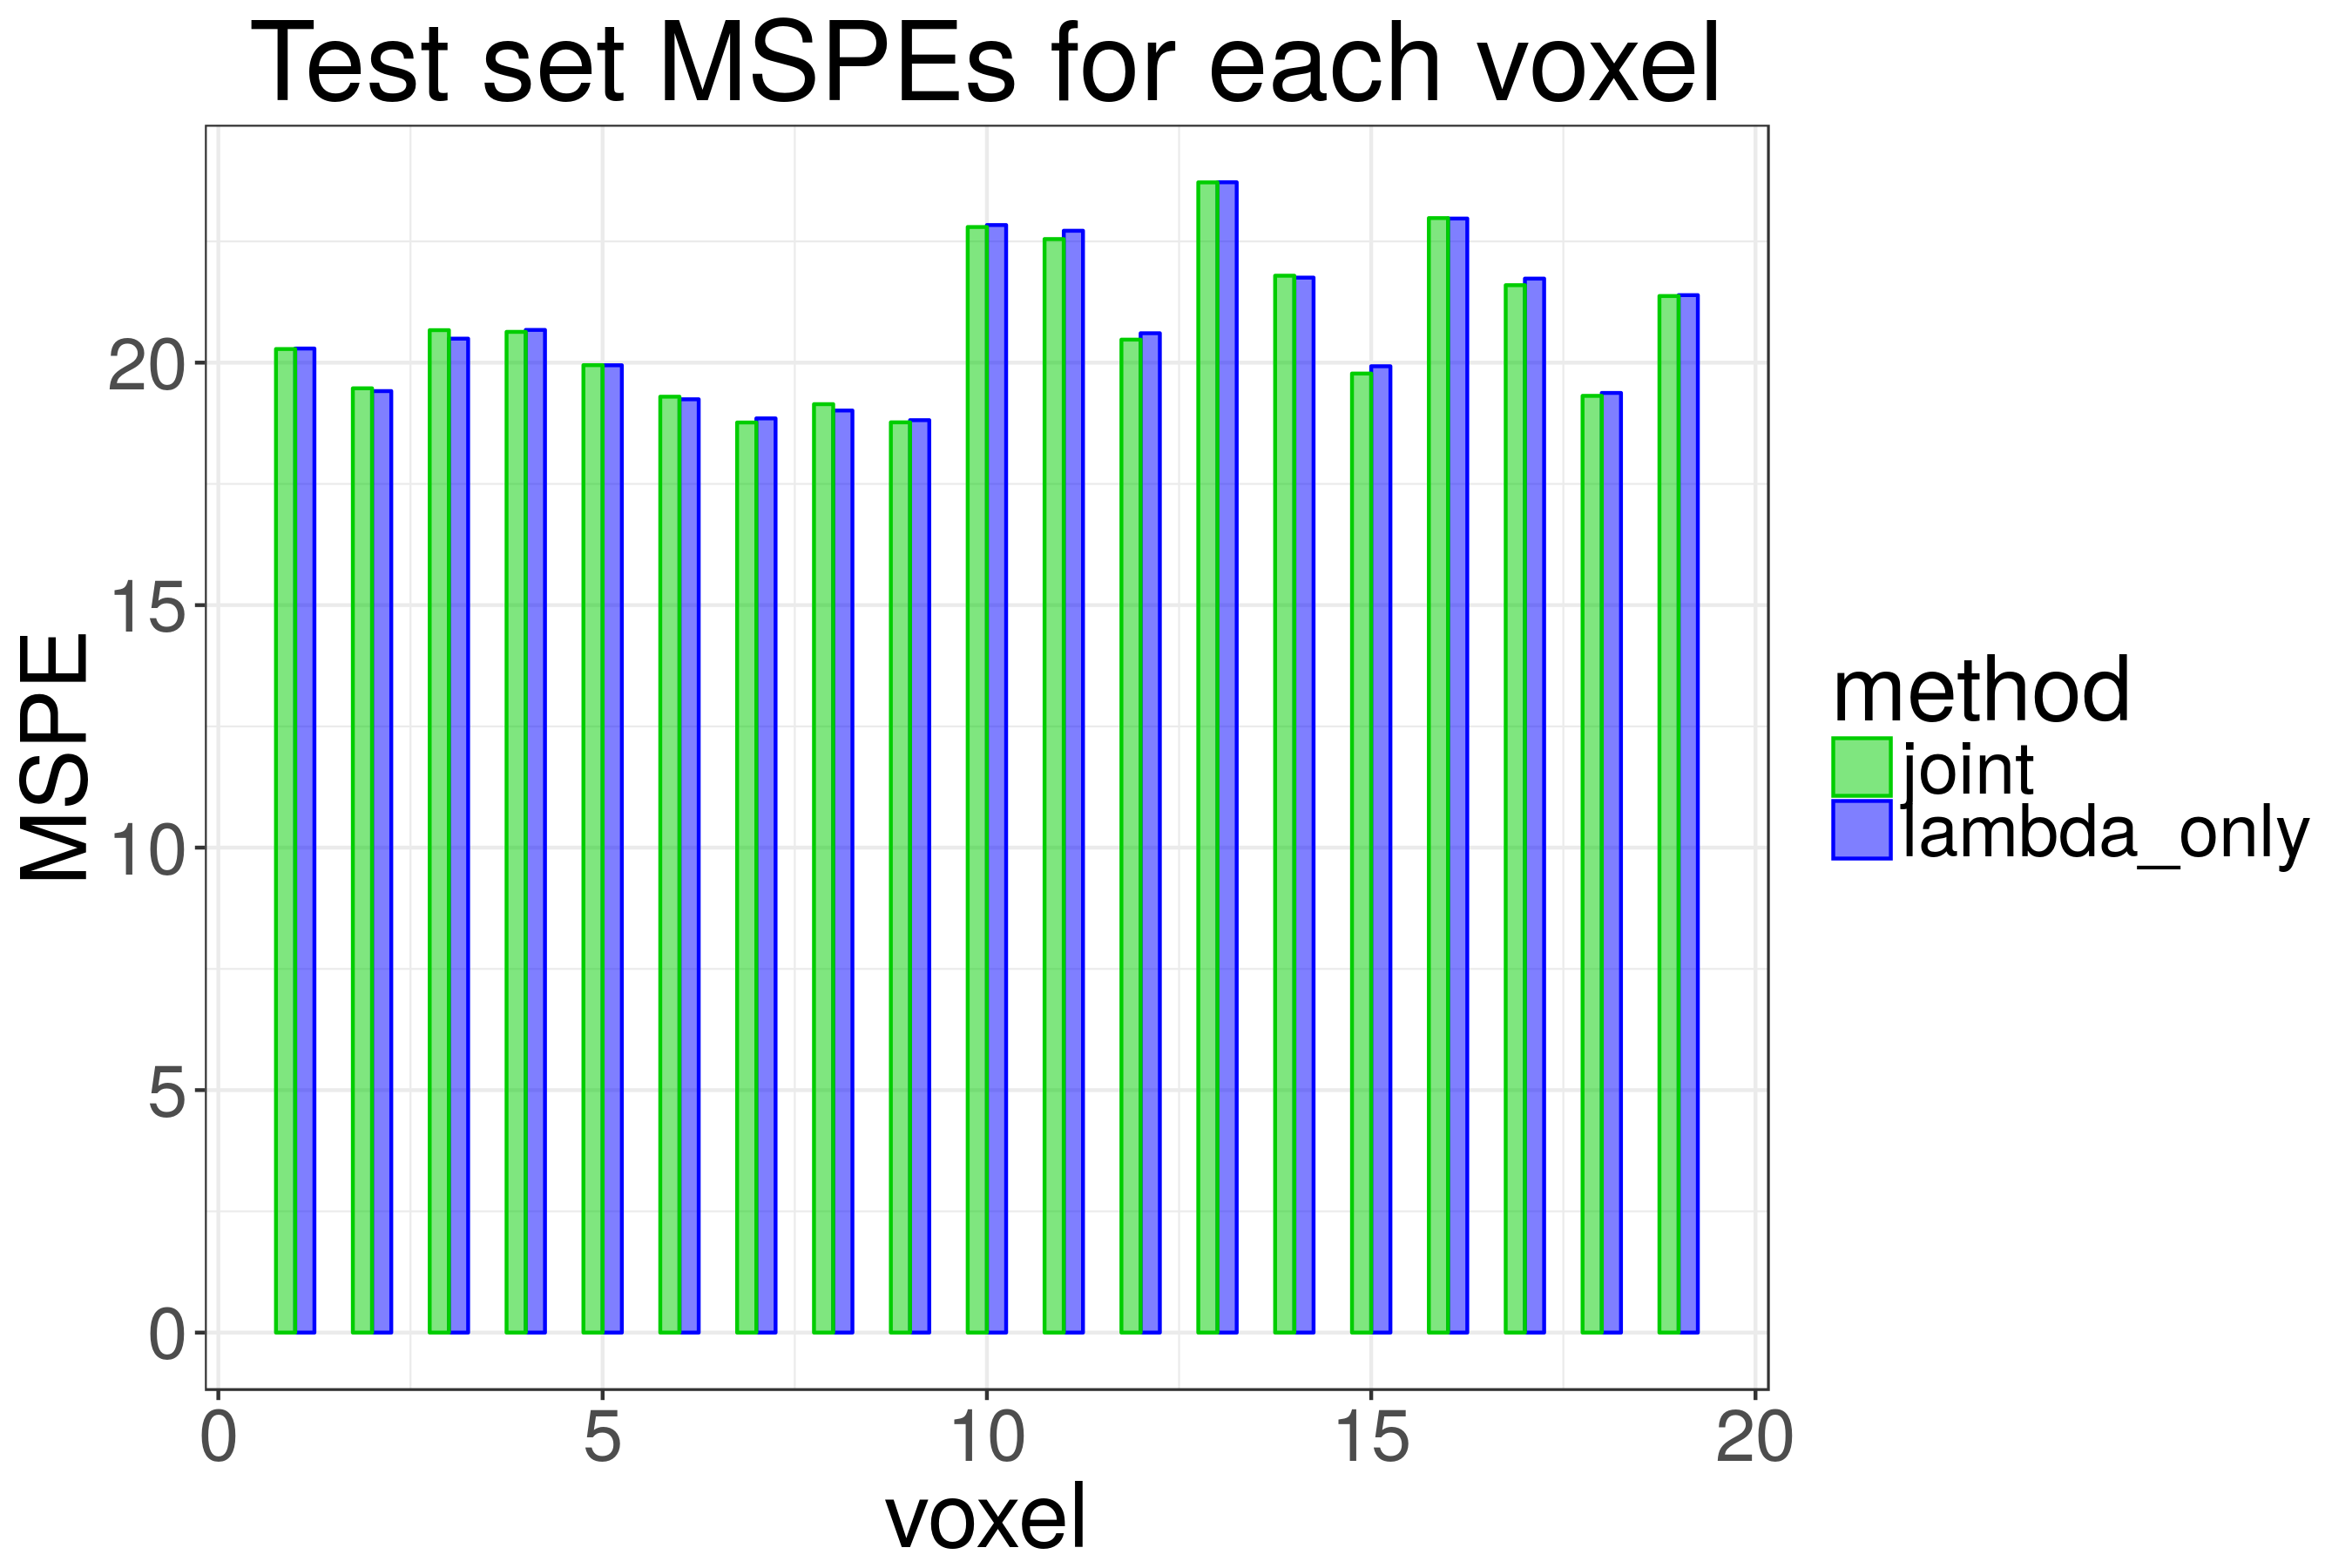
\includegraphics[width = \textwidth]{./single_response_fmri_figures/fmri_mspe.png}
	\end{subfigure}
  \caption{(a) $\text{slope}(y_{new}, \hat y)$ for each of the twenty voxels. Blue are slopes when predicting using
	LASSO with only $\lambda$ selection, while green are slopes when predicting using
	our method of jointly selecting $K$ and $\lambda$. (b) The MSPEs on the test data, again comparing the two methods.
	(voxel 20 was ignored in this plot, as both LASSO and and our method returned poor fits relative to the other voxels. )}
	\label{fig:fmri_single_response_results}
\end{figure}

As a particular example, in figure \ref{fig:fmri_single_response_results_scatter}, we look at the scatterplot of $y_{new}$ and $\hat y$ for voxel 15.
We can visually inspect that LASSO overshrinks the predictors (blue line), and choosing $K$ ameliorates this
over-shrinkage by re-inflating this prediction (green line).

\begin{figure}[!h]
	\centering
	\begin{subfigure}[t]{0.45\textwidth}
		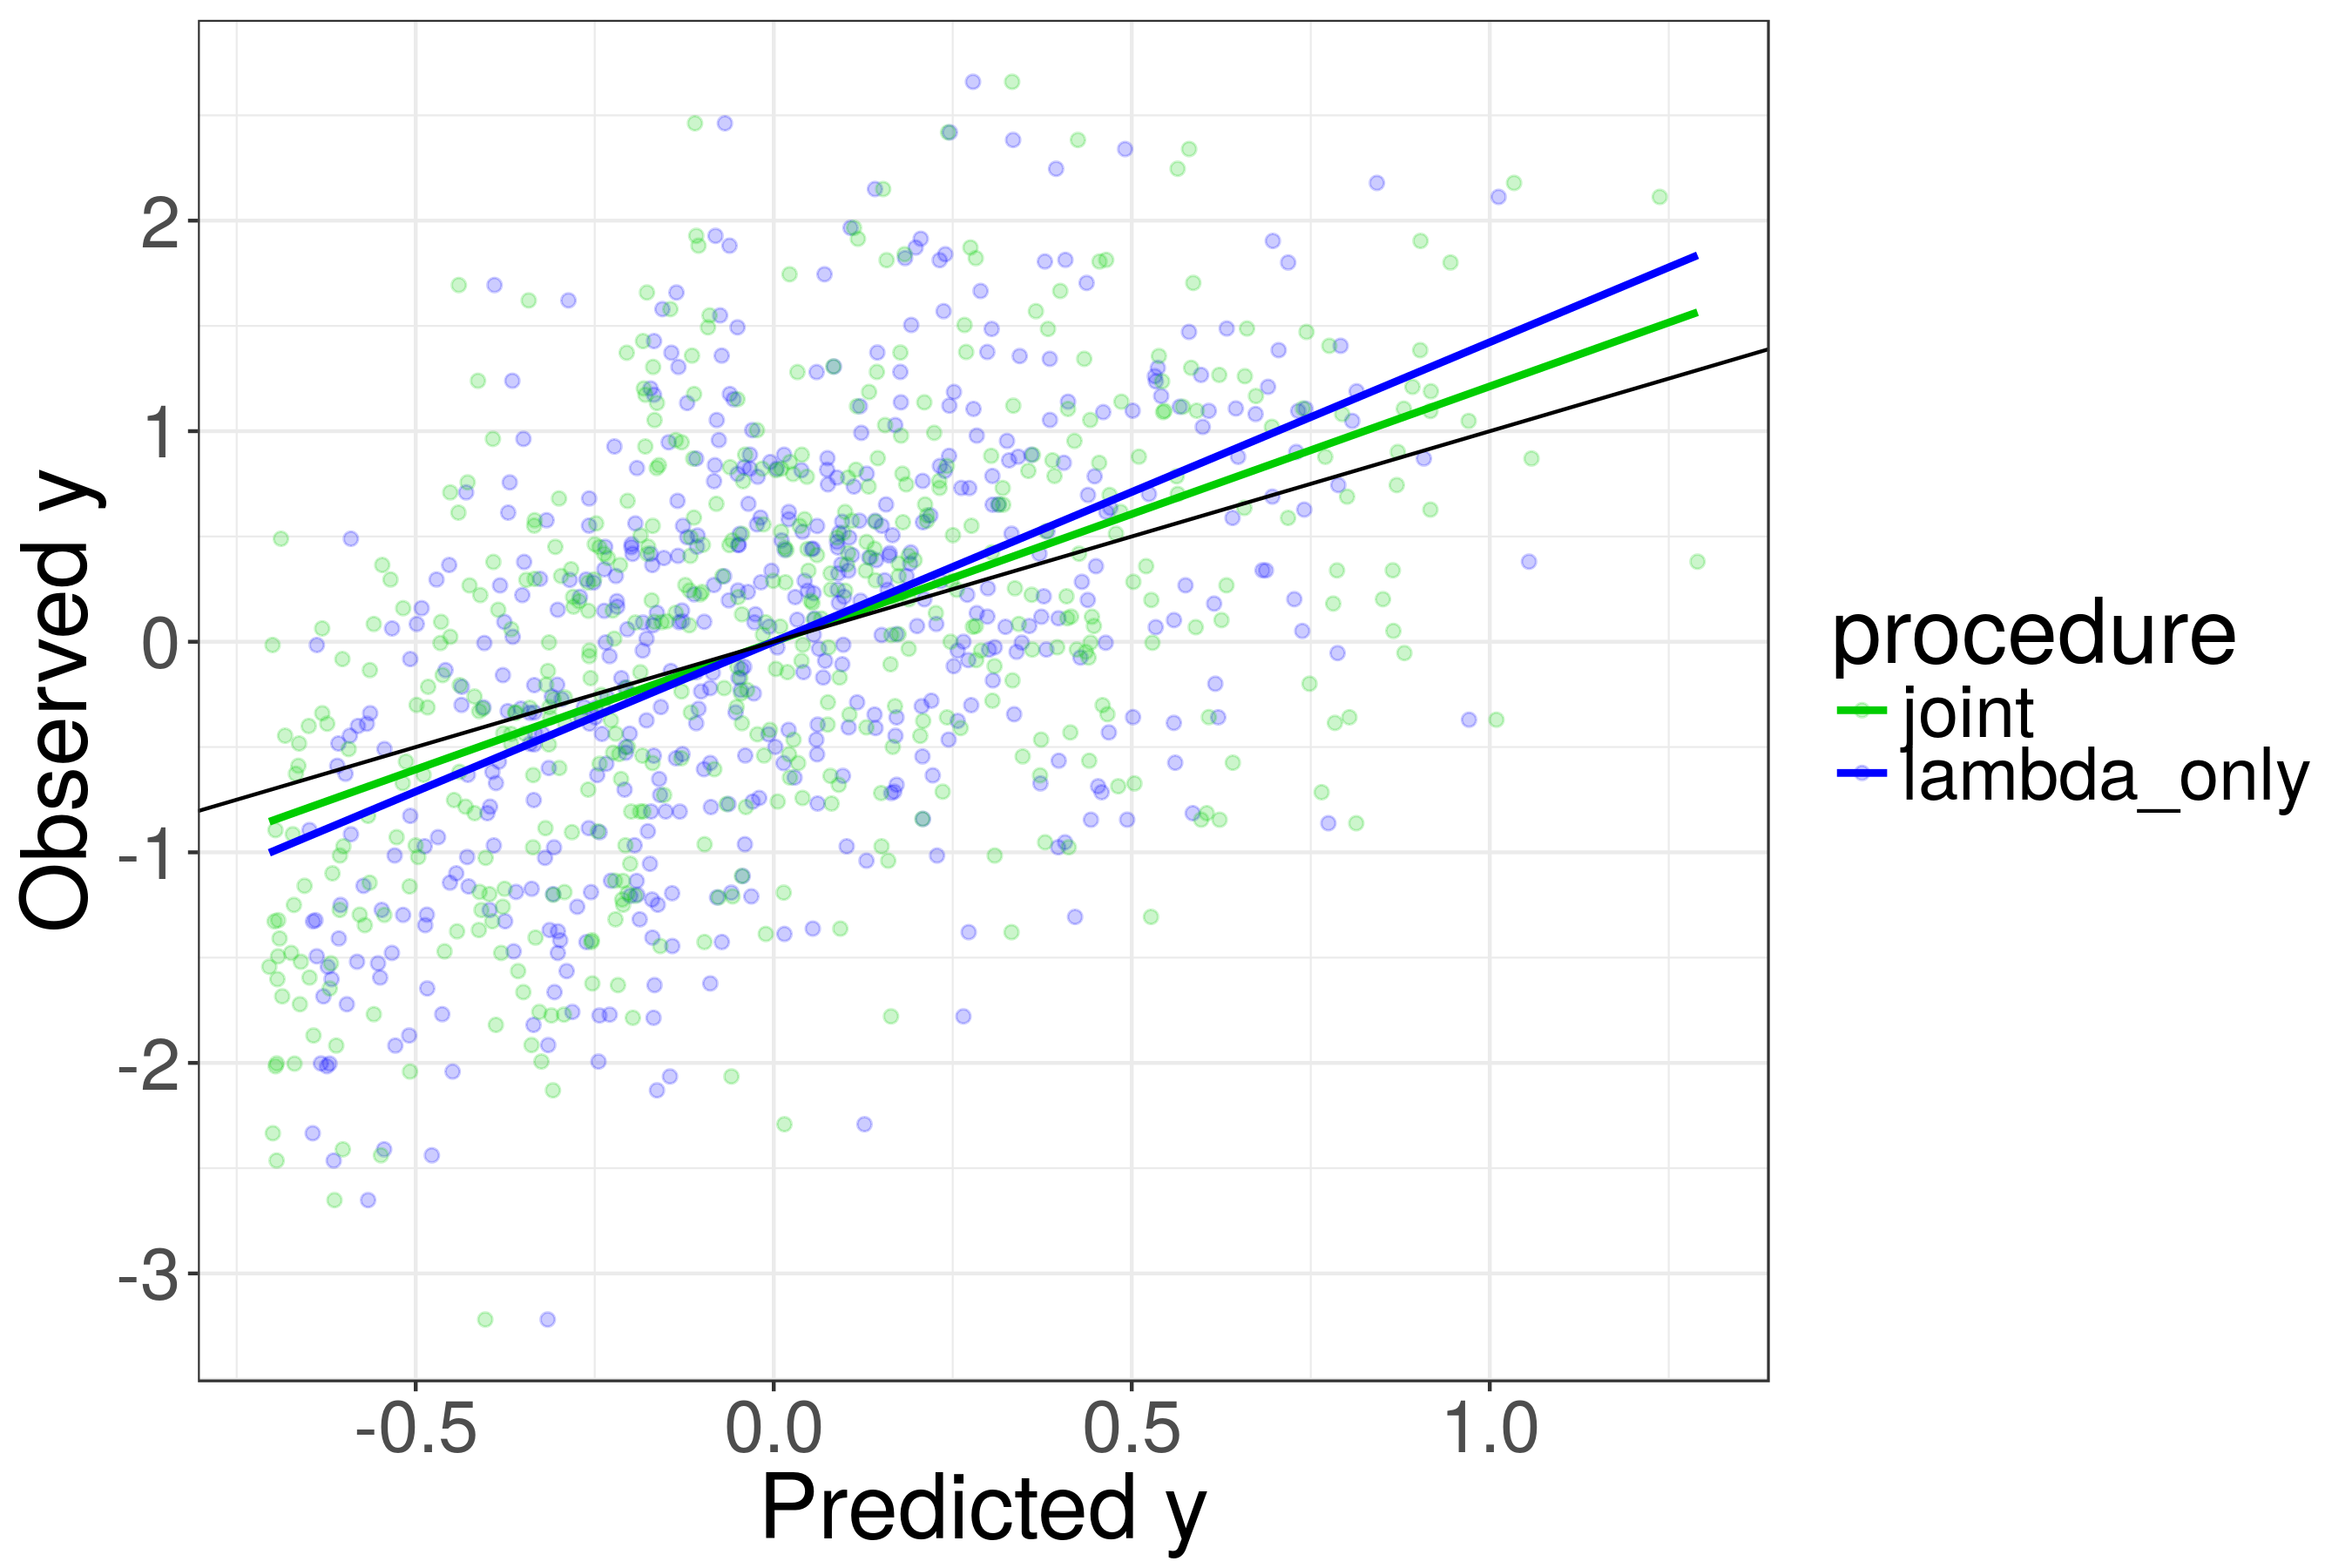
\includegraphics[width = \textwidth]{./single_response_fmri_figures/obs_y_vs_pred.png}
	\end{subfigure}
  \caption{Scatterplot of $(y_{new}, \hat y)$ in the test sample of voxel 15.
	Blue points are $\hat y$ computed with the LASSO objective, only choosing $\lambda$. Green points are $\hat y$
	computed with LASSO with $K$ selection joint with $\lambda$. Black line is the identity $y = x$ line.}
	\label{fig:fmri_single_response_results_scatter}
\end{figure}

We therefore conclude that for this particular data application, LASSO over-shrinks the predictors, and
it appears that choosing $K$ jointly with $\lambda$ in running LASSO can help pull the slopes back towards one.

For this particular analysis, we have treated each voxel as a separate regression problem. However,
we know that the responses of these voxels are correlated, and in the next section, we will consider shrinkage for
multi-response regression in a way that takes advantage of the relationship between these 20 voxels.

\end{document}
